\documentclass[11pt]{article}
\usepackage[margin=1in]{geometry}
\usepackage{amsmath,amssymb,amsthm}
\usepackage{bm}
\usepackage{graphicx}
\usepackage{booktabs}
\usepackage{multirow}
\usepackage{xcolor}
\usepackage[round]{natbib}
\usepackage[colorlinks=true,linkcolor=blue,citecolor=blue,urlcolor=blue]{hyperref}
\setlength{\emergencystretch}{3em}

\newtheorem{theorem}{Theorem}
\newtheorem{proposition}{Proposition}
\newtheorem{lemma}{Lemma}
\newtheorem{corollary}{Corollary}
\newtheorem{definition}{Definition}
\newtheorem{assumption}{Assumption}
\newtheorem{remark}{Remark}
\newcommand{\HHI}{\mathrm{HHI}}
\newcommand{\range}{\operatorname{range}}

\title{\textbf{Coalition Design under Heterogeneous AV Objectives: Regimes and Low-Regret Selection in Mixed-Autonomy Networks}}
\author{Luyao Niu \and Ruolin Li}
\date{\today}

\begin{document}
\maketitle

\begin{abstract}\sloppy
When several autonomous-vehicle (AV) operators share a road network, should
their routing be centralized, or should some independent decision centers be
retained? We study this question when operators have heterogeneous management
objectives, aggregate demand is fixed, and human-driven vehicles (HDVs)
continue to reroute. Each coalition is an atomic splittable player with a
convex management objective and member-level origin--destination obligations;
HDVs form a nonatomic Wardrop population. On a fixed affine support, we project
each coalition response onto its demand-feasible tangent and remove the
directions that HDVs can reproduce. The resulting activated response signature
is sufficient for aggregate equilibrium and minimal for the conditional
response map. It yields a general-network merge-direction score: stronger
coupling improves congestion exactly when the screened response has negative
system-cost projection. A canonical bottleneck theorem then identifies three
regimes. Coalition organization is neutral when HDVs fully screen the response;
centralization is favored when it moves effective response toward the relevant
boundary; and partial coordination can dominate both endpoints when the
system-cost-minimizing response is interior. We evaluate local merge policies
against complete four-company audit scans. In Sioux Falls, one- and two-step
policies attain an optimal arrangement in all four tested states, whereas an
always-grand rule loses up to $18.695$ recovery percentage points. Across 480
certified profiles on independent Braess and directed-grid networks, one-step
merging is exact in $29$ of $32$ states with mean regret $0.332$ points, while
two-step lookahead is exact in all $32$. Both networks move from grand to
partial coordination at high AV penetration under sufficiently strong
governance, although the transition boundary differs. Adding an explicit
governance burden generates grand, partial, and fragmented policy intervals.
HHI remains descriptive because it does not identify objective composition,
demand authority, or the response that survives HDV reallocation. The results
concern conditional continuation design, not endogenous coalition formation or
empirical calibration of operator objectives.
\end{abstract}

\noindent\textbf{Keywords:} mixed autonomy; coalition structure; heterogeneous AV management objectives; atomic splittable routing; Nash--Wardrop equilibrium; congestion; fleet organization

\section{Introduction}\label{sec:intro}

The transition to mixed-autonomy traffic creates an organizational problem in addition to a control problem. Autonomous vehicles (AVs) will be dispatched by multiple firms, platforms, or routing authorities, while human-driven vehicles (HDVs) continue to respond to congestion through individual route choice. The firms need not value the same operational outcome: one may emphasize the travel time of its own fleet, another may internalize a larger share of congestion, and a third may encode reliability, energy, or service obligations. The same set of firms can therefore be operated as independent routing centers, coordinated in partial coalitions, or placed under a common dispatcher. These arrangements are not equivalent when the aggregate demand and the physical road network are held fixed.

This paper studies the resulting design problem. Given a set of heterogeneous
AV companies, when should their routing be centralized, when should partial
independence be retained, and can a local rule select the organization without
relying on a full ex post enumeration of partitions? The question is
deliberately conditional. A partition and a governance rule are specified
before routing begins; companies retain the OD obligations associated with the
trips they have accepted; and the analysis compares the equilibria induced by
alternative arrangements. We do not model whether firms merge or sign an
agreement. The object of interest is the operational consequence of an
arrangement that a platform, fleet manager, or public authority could choose
among feasible alternatives.

The need for this distinction is practical as well as theoretical. Ownership concentration statistics such as the Herfindahl--Hirschman Index (HHI) summarize who controls how much mass and are used in market-screening contexts \citep{usdojftc2023}. They do not record what those firms optimize, which firms are grouped together, how many routing decision centers remain, which OD obligations each member must preserve, or which parts of a coalition response can be offset by HDV rerouting. Consequently, two organizations with the same company HHI, coalition size, and aggregate demand can induce different network flows. The conditional design problem can be written as
\begin{equation}
\Pi^\star(\alpha,\theta,\gamma)\in\arg\min_{\Pi\in\mathfrak P(N)}J\!\left(x^\star(\Pi;\alpha,\theta,\gamma)\right),
\label{eq:design-map-intro}
\end{equation}
where $\Pi$ is a feasible partition of the companies, $\gamma$ is a governance intensity, $\alpha$ is AV penetration, $\theta$ collects objective types, and $x^\star$ is the mixed-autonomy equilibrium induced by that arrangement. The map is a design object, not an endogenous coalition-formation equilibrium.

We implement this design problem as a coalition-structured mixed Nash--Wardrop game. Each coalition is an atomic splittable player with a convex management objective, while HDVs form a nonatomic Wardrop population. All vehicles experience the same physical edge cost; heterogeneity enters through the objectives used to manage AV flows. The main treatment uses identity-preserving coordination: members may jointly choose routes, but each member must satisfy its own accepted OD demand. Operational pooling, which relaxes those member-level constraints, is analyzed separately because it changes feasible authority rather than merely changing objective aggregation. The formulation links atomic congestion games and Cournot--Wardrop interaction \citep{haurie1985,orda1993,harker1988,boulogne2002} with multiclass assignment \citep{dafermos1972} and mixed-autonomy routing \citep{mehr2019,lazar2021,biyik2021}.

The model makes the transmission mechanism explicit. Demand conservation
restricts every coalition's route response to an OD-feasible tangent. After
this response is aggregated in edge space, HDVs can absorb any component that
lies in their own Wardrop adjustment space. The remaining component is the
activated coalition response. Projecting that response onto the gradient of
system travel time produces a directional test for a proposed merge. The
criterion distinguishes a screened regime, in which organization is locally
neutral, from regimes in which stronger coupling raises or lowers congestion.
In the canonical bottleneck, it also identifies an interior effective-response
target at which partial coordination can dominate both grand and singleton
organization.

Our first contribution is a unified representation of heterogeneous coalition control in mixed-autonomy routing. The model separates the physical cost function shared by all vehicles from the company management objective, the coalition governance matrix, the number of underlying companies $n$, and the number of active coalition decision centers $K=|\Pi|$. The convex quadratic family contains independent routing, partial cross-member internalization, and common-dispatcher arrangements while preserving the OD obligations needed for a clean coalition comparison.

Our second contribution is a regime theory for coalition design. Starting from
the bordered sensitivity systems used for equilibrium networks with
polyhedral constraints \citep{tobin1988,qiu1989,patriksson2004,josefsson2006},
we derive the OD-restricted coalition response, aggregate it in edge space,
and quotient it by the endogenous HDV Wardrop tangent. On a fixed affine
support, the activated response signature is sufficient for aggregate
equilibrium and minimal for the complete conditional response map. Its
system-cost projection gives a general-network merge-direction score. The
canonical bottleneck sharpens this score into a threshold theorem: complete
HDV screening makes organization neutral, a boundary regime favors changes
that reduce effective response, and an interior regime can favor partial
coordination. Parametric equilibrium computation supplies the complementary
support-traversal perspective \citep{klimm2025}.

Our third contribution is a certified, regret-based selection framework. We
evaluate one- and two-step agglomerative policies against complete
four-company scans, using enumeration only to audit the selected partitions.
Both policies attain a state optimum in all four Sioux Falls conditions. On
independent Braess and directed-grid networks, the one-step rule is exact in
$29$ of $32$ states with mean regret $0.332$ recovery points, while two-step
lookahead is exact in all $32$ states. Across the $480$ certified
cross-network profiles, grand coordination is preferred at lower penetration,
whereas partial coordination emerges at high penetration under sufficiently
strong governance on both topologies. An explicit governance-burden model
produces calculable intervals in which grand, partial, or fragmented control is
optimal. Composition sensitivity, company-count, spatial-exposure, and HHI
diagnostics establish why the policy must use the response state rather than a
mass statistic.

The numerical evidence is deliberately bounded. The three networks are
computational benchmarks, not an empirical sample of mobility markets. The
reported rankings hold within the declared objective family,
identity-preserving governance rule, demand portfolios, and route sets; the
affine regime results are not asserted as global BPR theorems. The two-step
policy's zero observed regret is a benchmark result rather than a universal
guarantee. Pricing, passenger acceptance, empty-vehicle repositioning,
platform profits, empirical calibration, and endogenous formation remain
outside the paper's scope.

The remainder of the paper follows this logic. Section~\ref{sec:model} defines
the physical network, company objectives, coalition governance, equilibrium,
and performance measures. Section~\ref{sec:response} establishes
well-posedness, the activated response, the general merge score, and the
canonical regimes. Section~\ref{sec:ownership} interprets coalition
composition, governance burden, HHI, and the boundary between objective
coordination and pooling. Section~\ref{sec:experiments} reports mechanism,
regret, and cross-network evidence. Section~\ref{sec:discussion} discusses
implementation and scope, and Section~\ref{sec:conclusion} summarizes the
bounded implications.

\section{Positioning in the Literature}\label{sec:related-work}

\subsection{Multiple operators and mixed-autonomy networks}

Research on automated mobility-on-demand and ride-sourcing has established that several operators can compete for demand while interacting through congestion. Existing formulations study operator competition and market decisions \citep{turan2022,wang2022amod}, jointly model ride-hailing competition with transit planning \citep{wei2022}, or embed ride-sourcing services in urban traffic-network equilibrium \citep{xu2021ridesourcing}. A related control literature studies the equilibrium and incentive consequences of routing AVs alongside individually routed vehicles \citep{mehr2019,lazar2021,biyik2021}. These strands motivate the distinction between positive-mass controlled flows and nonatomic HDVs, but they leave a different organizational question open: conditional on fixed demand, how should heterogeneous routing objectives be grouped into independent or coordinated decision centers? Operator count or market share alone does not answer that question, because it does not specify objective composition, coalition governance, or member-level OD authority. The present paper isolates that operational layer while holding the physical road-cost function common across vehicle classes.

\subsection{Atomic congestion games, collusion, and coalition structure}

Atomic congestion and Nash--Wardrop models provide the natural language for positive-mass routing authorities whose choices affect the costs faced by other users \citep{haurie1985,orda1993,harker1988,boulogne2002}. Multiclass assignment and strategic routing further show how equilibrium depends on the interaction between populations with different decision rules \citep{dafermos1972,cominetti2009}. Work on collusion and concentration in congestion games demonstrates that changing the strategic grouping of users can alter equilibrium efficiency \citep{hayrapetyan2006,roughgarden2002}. The gap relevant here is not the existence of coalition effects; it is their identification in a mixed-autonomy network with heterogeneous company objectives and fixed OD obligations. A coalition in our model is therefore more than a larger atomic mass. Its governance matrix determines which member effects are internalized, while the partition determines how many strategic response centers remain. This distinction allows the same company masses and coalition HHI to produce different continuation equilibria.

\subsection{Equilibrium sensitivity and the transmission of organizational change}

Sensitivity analysis for equilibrium network flows uses active supports, bordered systems, and derivatives restricted to polyhedral feasible sets \citep{tobin1988,qiu1989,patriksson2004,josefsson2006}. Recent work on atomic splittable games addresses the complementary computational problem of locating and traversing parametric equilibrium supports \citep{klimm2025}. We use these tools for their established purpose and do not present the bordered inverse as a new numerical primitive. The paper's addition is to compose three response blocks that are usually kept separate: the OD-restricted response of each coalition, its edge-space aggregation, and the endogenous HDV Wardrop adjustment space. The resulting activated signature identifies the part of an organizational change that can reach aggregate congestion on a fixed support. This composition is also why scalar concentration summaries need not order network outcomes: the same coalition-side displacement can be fully screened in one HDV support and remain active in another.

\subsection{Ownership, information, and interoperability}

Ownership and information architecture are related institutional choices but are not interchangeable operational mechanisms. HHI is an ownership-concentration statistic used in merger screening \citep{usdojftc2023}; information-design studies show that changing what users know can itself alter network congestion and need not improve it monotonically \citep{acemoglu2018,massicot2022}. Transport policy and data-system work likewise treats interoperability as a coordination standard that can be implemented without common ownership \citep{marquez2025,ec2023mobilitydataspace}. These sources motivate a separation that is central to our design interpretation. Identity-preserving coalition coordination changes the aggregation of management objectives at fixed member authority; operational pooling changes the feasible authority by relaxing member-level OD constraints; and information sharing is a possible microfoundation for better response estimation, not a guarantee of lower network travel time. The paper keeps these channels separate in both the model and the experiments.

\subsection{Position of this paper}

The literature supplies the ingredients for our analysis but does not connect
them to a regime and selection theory for coalition organization. We combine
atomic coalition control, mixed-autonomy equilibrium, and support-conditional
sensitivity in a model with common physical costs and heterogeneous AV
management objectives. The activated response yields a general-network merge
score and a canonical threshold at which partial coordination can dominate
both endpoints. Complete partition scans then serve as audit baselines for
local policies with measurable regret, while governance burden produces
explicit organizational intervals. The resulting claim is operational and
bounded: coalition design matches a response state, whereas HHI and coalition
size remain descriptors rather than sufficient equilibrium controls.

\section{A Regulator-Selected Coalition-Structured Routing Game}\label{sec:model}

The model separates a regulator's temporary coalition-design decision from the routing continuation equilibrium. In an emergency state, the regulator selects a feasible partition of AV companies and a coordination intensity; conditional on that institutional arrangement, each coalition routes its members' accepted requests as an atomic splittable player, while human-driven vehicles (HDVs) form a Wardrop population. The regulator does not reassign orders or prescribe vehicle-level routes. Four objects must remain distinct: physical link cost is a property of the road; a coalition routing objective governs dispatch; a company's realized accounting cost is an optional diagnostic; and coalition governance cost records the resources required to operate the temporary agreement. The partition is therefore an externally selected continuation-design treatment, not an endogenous formation equilibrium.

\subsection{Network, routes, and fixed demand}\label{sec:model_network}

Traffic uses a finite directed graph $G=(V,E)$ and a finite set $W$ of origin--destination (OD) pairs. For each $w\in W$, total demand $d_w>0$ is fixed and the admissible route set is $\mathcal R_w$. Let $\mathcal R=\bigcup_{w\in W}\mathcal R_w$, and let $\delta_{er}=1$ if edge $e$ belongs to route $r$. For any population, route flows $f$ induce edge flow
\begin{equation}\label{eq:route-edge-map}
 x_e=\sum_{r\in\mathcal R}\delta_{er}f_r.
\end{equation}
Every vehicle experiences the same physical link cost $c_e(x_e)$. This common-cost assumption is what makes AV governance a behavioral mechanism rather than a vehicle-class-specific road technology. The numerical model uses the Bureau of Public Roads function
\begin{equation}\label{eq:bpr}
 c_e(x_e)=t_e^0\left[1+B\left(\frac{x_e}{\kappa_e}\right)^\eta\right],
 \qquad B=0.15,\quad \eta=4,
\end{equation}
where $t_e^0$ is free-flow time and $\kappa_e$ is capacity. The theoretical results require only that $c_e$ be continuous and nondecreasing; affine results use
\begin{equation}\label{eq:affine}
 c_e(x_e)=a_e+b_ex_e,\qquad b_e\geq0.
\end{equation}
The experienced cost of route $r$ is $C_r(x)=\sum_{e\in E}\delta_{er}c_e(x_e)$. The BPR specification is used for numerical continuation experiments; it is not used to claim the affine closed form below.

\subsection{Wildfire-disrupted application state}\label{sec:model_hazard}

The coalition model is evaluated under an exogenous emergency network state. For hazard scenario $\omega$ and decision epoch $t$, let $E_t^\omega\subseteq E$ be the set of open roads. A closed road is removed from the admissible route set. An open but degraded road has state-dependent free-flow time $t_{e,t}^{0,\omega}$, capacity $\kappa_{e,t}^\omega$, and an optional public risk attribute $r_{e,t}^\omega$. Its physical cost is
\begin{equation}\label{eq:hazard-bpr}
 c_{e,t}^\omega(x_e)=t_{e,t}^{0,\omega}\left[1+B\left(\frac{x_e}{\kappa_{e,t}^\omega}\right)^\eta\right].
\end{equation}
The first application implementation uses static hazard snapshots, so $t$ is suppressed within one continuation solve. A rolling-horizon update is a later extension rather than a maintained assumption of the fixed-support response theorem.

The total flow on an open edge is
\begin{equation}\label{eq:hazard-flow-decomposition}
 x_{e,t}^\omega=u_{e,t}^\omega+h_{e,t}+\sum_{i\in N}f_{e,t}^i,
\end{equation}
where $u^\omega$ is optional exogenous background traffic, $h$ is ordinary HDV flow, and $f^i$ is commercial AV order flow. The HDV population is not an evacuation population: it observes public road and closure information, is responsive through the Wardrop block, and is not directly controlled by the regulator. Hazard risk can enter public generalized route cost as a fixed edge attribute; it does not by itself create a new vehicle class.

The emergency application may designate a set $E_{\mathrm{critical}}^\omega$ of roads whose capacity should be preserved for emergency-sensitive network access. This set enters the regulator's ex post evaluation or a declared capacity-protection constraint. The paper does not model household evacuation demand, rescue dispatch, shelter assignment, or resident-level evacuation behavior.

\subsection{Companies, AV demand, and coalition partitions}\label{sec:model_companies}

Let $N=\{1,\ldots,n\}$ be the underlying AV companies. Company $i$ controls an accepted OD-demand vector $d^i=(d_w^i)_{w\in W}$ and mass $m_i=\sum_wd_w^i$. HDV demand is $d^H=(d_w^H)_{w\in W}$, and the realized demand batch satisfies
\begin{equation}\label{eq:company-demand}
 d_w^H+\sum_{i\in N}d_w^i=d_w,\qquad w\in W.
\end{equation}
The routing stage is conditional on this accepted batch. Request acceptance, pricing, passenger platform choice, empty-vehicle repositioning, and inter-batch balancing are outside the model. Thus a company can change the path of an assigned request but cannot change its OD pair during the routing game. Holding the batch fixed is deliberate: it lets the comparisons identify routing and governance effects without conflating them with market-share or demand-formation effects.

A coalition structure is a partition $\Pi=\{C_1,\ldots,C_K\}$ of $N$, where $K=|\Pi|$ is the number of independent routing decision centers. The regulator selects $\Pi$ from a declared feasible menu $\mathfrak P(N)$; conditional on $\Pi$, its blocks are the routing players. The number $n$ of underlying companies and the number $K$ of active coalitions are distinct: changing $n$ changes the population of objectives, whereas changing $K$ changes which objectives are jointly optimized. Company-level HHI is a function of the $m_i$; coalition-level HHI is a function of the aggregate masses $m_C=\sum_{i\in C}m_i$. Neither index defines a coalition's management objective or a voluntary formation payoff.

For company $i$, let $y^i$ denote its route-flow vector and let $\Lambda_i$ map routes to company edge flows. A coalition $C$ may use the stacked member vector $y^C=(y^i)_{i\in C}$. Under the main identity-preserving governance rule, every member retains its own OD obligation:
\begin{equation}\label{eq:identity-feasible}
 \mathcal Y_C^{\mathrm{id}}=
 \left\{y^C\geq0:\Gamma_Cy^C=d^C\right\},
 \qquad
 \Gamma_C=\operatorname{blkdiag}(\Gamma_i)_{i\in C}.
\end{equation}
The coalition jointly chooses $y^C$ but cannot reassign an accepted passenger obligation from one member to another. This is the main treatment because it changes the decision maker while holding ownership of requests fixed; the resulting comparison isolates objective aggregation and coordination from a change in service authority.

An operational-pooling governance rule instead preserves only the coalition total on each OD pair:
\begin{equation}\label{eq:pool-feasible}
 \mathcal Y_C^{\mathrm{pool}}=
 \left\{y^C\geq0:\sum_{i\in C}\sum_{r\in\mathcal R_w}y_r^i
 =\sum_{i\in C}d_w^i,\ \forall w\right\}.
\end{equation}
Pooling is a separate intervention because it changes the feasible set, whereas identity-preserving coordination changes only the objective aggregation and cross-member internalization. The distinction matters empirically: a pooling result cannot be interpreted as evidence about coordination alone when pooling also permits one member to serve another member's accepted demand.

\begin{proposition}[Pooling changes feasible authority]\label{prop:pooling}
For every coalition $C$, $\mathcal Y_C^{\mathrm{id}}\subseteq\mathcal Y_C^{\mathrm{pool}}$. The inclusion can be strict. If all members have identical admissible routes for every OD pair and the coalition objective depends only on aggregate coalition flow, the two sets induce the same aggregate route-flow set.
\end{proposition}

\begin{proof}
Summing the member-specific equalities in \eqref{eq:identity-feasible} gives the pooled equalities in \eqref{eq:pool-feasible}. Hence the identity-preserving set is contained in the pooling set. The inclusion is strict whenever a pooled solution allocates more than $d_w^i$ of OD-$w$ flow to member $i$. Conversely, if all members share the same route set, any pooled aggregate route vector $\bar y_w$ can be split as $y_w^i=(d_w^i/d_w^C)\bar y_w$, where $d_w^C=\sum_{i\in C}d_w^i$. This split satisfies every member equality and produces the same aggregate vector. If the objective depends only on that aggregate vector, the induced aggregate optimization problems coincide.
\end{proof}

\subsection{Company management objectives}\label{sec:model_objectives}

Let $F_e^C=\Lambda_Cy^C$ be coalition $C$'s edge flow and $x_e^{-C}=x_e-F_e^C$ be the flow controlled by other populations. The coalition management objective is
\begin{equation}\label{eq:coalition-objective}
 \Phi_C(y^C;y^{-C},h)
 =\sum_{e\in E}\int_0^{F_e^C}c_e(x_e^{-C}+s)\,ds
 +\Psi_C(y^C).
\end{equation}
The first term is the common physical routing component. It is written as an integral because, conditional on the other populations' flow, its derivative with respect to coalition flow is the experienced link cost $c_e(x_e)$. This gives the coalition the correct marginal road delay while preserving a convex objective whenever $c_e$ is nondecreasing. The convex function $\Psi_C$ is the company- and governance-specific management objective. It may represent own-fleet congestion internalization, energy, reliability, service commitments, route preferences, or cross-member coordination. These interpretations are alternative economic readings of the same reduced-form routing objective; the numerical design below uses the congestion-curvature component and does not claim to estimate each interpretation separately.

The route marginal field used by coalition $C$ is
\begin{equation}\label{eq:coalition-gradient}
 G_C(y)=\nabla_{y^C}\Phi_C
 =\Lambda_C^\top c(x)+\nabla\Psi_C(y^C).
\end{equation}
HDVs use $G_H(y,h)=\Lambda_H^\top c(x)$.

For the exact response analysis, use a convex quadratic management objective:
\begin{equation}\label{eq:quadratic-objective}
 \Psi_C(y^C)=\frac12(y^C)^\top H_Cy^C+q_C^\top y^C,
 \qquad H_C=H_C^\top\succeq0.
\end{equation}
The matrix $H_C$ is the curvature of the coalition's management objective on route flows, and $q_C$ contains fixed marginal operating costs or route-specific priorities. Positive semidefiniteness is the modeling restriction that rules out locally concave management incentives; strict curvature is imposed only on the feasible OD-preserving tangent when a unique response is needed. The earlier perceived-slope model is nested by
\begin{equation}\label{eq:slope-nested}
 H_C=\Lambda_C^\top\operatorname{diag}(\widehat\theta^C)\Lambda_C,\qquad q_C=0.
\end{equation}
Thus $\widehat\theta_e^C$ is an edge-separable parameterization of objective curvature, not the complete company objective. In particular, it should not be read as a measured coefficient of the BPR road function.

Under identity-preserving coordination, collect member edge flows on edge $e$ in $\bm f_{C,e}=(f_e^i)_{i\in C}$. We parameterize governance by
\begin{equation}\label{eq:governance-matrix}
 \Psi_C(y^C)=\frac12\sum_{e\in E}\bm f_{C,e}^{\top}\Omega_{C,e}\bm f_{C,e}+q_C^\top y^C,
 \qquad \Omega_{C,e}=\Omega_{C,e}^{\top}\succeq0.
\end{equation}
The diagonal entries of $\Omega_{C,e}$ describe company-specific curvature. The off-diagonal entries describe the degree to which the coalition internalizes congestion interactions between members. This matrix is therefore a governance object: it changes whose marginal routing consequences are included in a decision, while the physical cost $c_e$ remains unchanged.

For the main coalition-composition experiment, let $\tau_i>0$ be a company objective type and let $\bar b_e\geq0$ be a fixed reference curvature. We use
\begin{equation}\label{eq:gamma-governance}
 \Omega_{C,e}(\gamma)=\bar b_eD_C^{1/2}
 \left[(1-\gamma)I_C+\gamma\mathbf1_C\mathbf1_C^\top\right]
 D_C^{1/2},
 \qquad D_C=\operatorname{diag}(\tau_i)_{i\in C},\quad \gamma\in[0,1].
\end{equation}
The scalar $\gamma$ is a governance parameter, not an information-quality estimate or an empirically calibrated technology parameter. At $\gamma=0$, companies retain only their own diagonal management curvature. At $\gamma>0$, the coalition internalizes cross-member interactions, with the same member types $\tau_i$ and reference slopes $\bar b_e$. The path is chosen so that increasing coordination adds off-diagonal terms without changing the sign of the curvature matrix; this makes comparative statics interpretable as a change in governance rather than a loss of well-posedness.

\begin{proposition}[Convex governance path and inert partition labels]\label{prop:governance}
The matrix $\Omega_{C,e}(\gamma)$ is positive semidefinite for every $\gamma\in[0,1]$. Under identity-preserving constraints, if $\gamma=0$ and $(\tau_i,q_i,d^i,\Lambda_i)$ are fixed, changing the coalition partition does not change the VI operator or its equilibrium set.
\end{proposition}

\begin{proof}
For any vector $v$,
\[
 v^\top\Omega_{C,e}(\gamma)v
 =\bar b_e(1-\gamma)\|D_C^{1/2}v\|^2
 +\bar b_e\gamma(\mathbf1_C^\top D_C^{1/2}v)^2\geq0.
\]
At $\gamma=0$, the management penalty is the sum of company-specific quadratic terms regardless of the coalition block in which each company is placed. Identity-preserving feasible sets are the same product of member-level OD polytopes for every partition, and the common physical term depends only on total edge flow. Therefore both the feasible set and stacked operator are unchanged.
\end{proof}

The positive-semidefinite statement does not by itself imply positive curvature on every OD-feasible coalition tangent. In particular, at $\gamma=1$ the governance matrix has rank one before it is combined with the route-incidence map. The fixed-support response theorem therefore applies only when its tangent-curvature condition is checked for the realized coalition and support; numerical BPR profiles remain certified by their VI and omitted-route tests rather than by this affine tangent theorem.

\subsection{Mixed Nash--Wardrop continuation equilibrium}\label{sec:model_equilibrium}

Let $h$ be HDV route flow and define
\begin{equation}\label{eq:feasible}
 \mathcal Z_\Pi=\left\{((y^C)_{C\in\Pi},h): y^C\in\mathcal Y_C,\ h\geq0,\ \Gamma_Hh=d^H\right\}.
\end{equation}

\begin{definition}[Heterogeneous-coalition mixed Nash--Wardrop equilibrium]\label{def:eq}
A feasible profile $z^*=((y^{C*})_{C\in\Pi},h^*)$ is an equilibrium for $(\Pi,\mathcal G)$ if every coalition minimizes \eqref{eq:coalition-objective} over its feasible set given other populations, while HDVs use only minimum experienced-cost routes within each OD pair. Equivalently, if $\mathcal F_\Pi$ stacks $G_C$ for all coalitions and $G_H$, then
\begin{equation}\label{eq:VI}
 \mathcal F_\Pi(z^*)^\top(z-z^*)\geq0
 \qquad\text{for all }z\in\mathcal Z_\Pi.
\end{equation}
\end{definition}

This is a finite-player Nash game coupled to a nonatomic Wardrop population. The general behavioral formulation does not require a common potential. Under the symmetric positive-semidefinite fixed-reference governance family used in the numerical experiments, however, the continuation operator is the gradient of the convex potential
\begin{equation}\label{eq:potential}
 \mathcal P_\Pi(y,h)=\sum_{e\in E}\int_0^{x_e}c_e(u)\,du+\sum_{C\in\Pi}\Psi_C(y^C).
\end{equation}
The coalition block is a best-response condition because the objective is convex in its own flow; the HDV block is Wardrop's equal-cost condition. The same physical cost $c_e$ couples all populations, while $H_C$, $q_C$, $\Gamma_C$, and $d^C$ encode organizational heterogeneity. The BPR experiments use a fixed reference curvature in $\Psi_C$ and should not be interpreted as the exact nonlinear own-travel-time atomic game.

Because the regulator compares different partitions, a continuation-selection rule is required whenever route-flow equilibrium is not unique. Let
\begin{equation}\label{eq:continuation-selection}
 z^\sigma(\Pi)\in\operatorname{SOL}(\mathcal F_\Pi,\mathcal Z_\Pi)
\end{equation}
denote a deterministic, commonly known selection for every $\Pi\in\mathfrak P(N)$. Aggregate edge flow is unique under the conditions in Proposition~\ref{prop:coalition-monotone}, but the rule is retained because member-level route flows may enter optional accounting diagnostics. The reported design comparisons are conditional on the same rule $\sigma$.

\subsection{Optional company accounting costs}\label{sec:model_private_costs}

The coalition routing objective $\Phi_C$ determines a continuation best response, but it is not itself an individual company accounting cost. Its integral term is a device for producing the desired marginal road-cost field, and its off-diagonal governance terms cannot generally be assigned uniquely to individual members. We therefore evaluate firm $i$ at a realized profile $z$ by the additive accounting cost
\begin{equation}\label{eq:individual-accounting-cost}
 \ell_i(z)
 :=\sum_{e\in E}f_e^i c_e(x_e)
 +\frac12\sum_{e\in E}\bar b_e\tau_i(f_e^i)^2
 +q_i^\top y^i.
\end{equation}
The first term is experienced fleet travel time, the second retains the firm's own management-curvature charge, and the third collects fixed marginal operating costs. Cross-member terms in $\Omega_{C,e}$ affect $\ell_i$ indirectly by changing the continuation flow, but they are not counted again as realized operating cost.

Operating a coalition can additionally require contracting, data integration, monitoring, or joint-dispatch resources. For the declared parametric family, define
\begin{equation}\label{eq:coalition-governance-cost}
 G_C(\kappa,\chi)
 :=\kappa\binom{|C|}{2}
 +\chi\sum_{\{i,j\}\subseteq C}(\tau_i-\tau_j)^2,
 \qquad \kappa,\chi\geq0,
\end{equation}
with $G_{\{i\}}=0$. The first component charges for each integrated company pair; the second allows heterogeneous objectives to be more costly to reconcile. These are transparent regulator-side governance-cost primitives rather than estimated costs. Given the selected continuation equilibrium, coalition $C$'s accounting value is
\begin{equation}\label{eq:coalition-private-value}
 K_C(\Pi;\sigma)
 :=\sum_{i\in C}\ell_i\bigl(z^\sigma(\Pi)\bigr)+G_C(\kappa,\chi),
 \qquad
 v(C,\Pi;\sigma):=-K_C(\Pi;\sigma).
\end{equation}
The dependence on the full partition is substantive: other coalitions and HDVs reroute when $\Pi$ changes. These accounting values are reported as diagnostics for the regulator's design problem; they are not evidence of voluntary coalition stability.

\subsection{System benchmark and scope}\label{sec:model_metrics}

Network congestion is measured by total system travel time
\begin{equation}\label{eq:J}
 J(x)=\sum_{e\in E}x_ec_e(x_e).
\end{equation}
Let $J^{UE}$ be the all-nonatomic Wardrop benchmark and $J^{SO}$ the system-optimal value for the same aggregate OD demand. We report normalized recovery
\begin{equation}\label{eq:rho}
 \rho=\frac{J^{UE}-J^{eq}}{J^{UE}-J^{SO}}.
\end{equation}
The statistic measures the fraction of the recoverable congestion gap closed relative to the two benchmarks. It is a system-performance statistic, not an individual company payoff, and it does not include governance resources, operating profit, passenger surplus, reliability, or distributional effects.

For descriptive comparison only, company HHI is
\begin{equation}\label{eq:hhi}
 \mathrm{HHI}_{\mathrm{firm}}=\sum_{i\in N}\left(\frac{m_i}{\sum_jm_j}\right)^2,
\end{equation}
and coalition HHI is defined analogously using $m_C$. These indices summarize mass concentration but omit objective curvature, OD portfolios, route access, cross-member governance, and HDV adjustment.

\paragraph{Information structure.}
The continuation benchmark is steady-state and complete-information with respect to the declared public network state: HDVs observe public experienced-cost and closure information and choose routes but are not directly controlled; each coalition observes the member-level flows and objective parameters required by its governance contract; and the regulator observes the declared company masses, accepted OD obligations, network state, and governance menu when comparing partitions. Information error and delayed public road information are robustness treatments, not assumptions of the baseline. The hazard state itself is exogenous to the routing game.

\paragraph{Standing assumptions.}
The accepted demand batch, route sets, and physical costs are fixed within each continuation episode. Physical costs are continuous and nondecreasing. Each coalition management objective is continuously differentiable and convex in its own route flow. The main continuation theorem further assumes affine physical costs, a fixed active support, full-row-rank OD constraints, positive curvature on every OD-feasible coalition tangent, and a nonredundant HDV tangent after zero-slope directions are removed. These additional conditions are exactly the conditions needed for the projected linear response; they are not imposed on the BPR numerical game. The regulator's temporary coordination authority and the common continuation-selection rule are institutional assumptions. Pricing, demand induction, passenger choice, capacity changes, and inter-episode repositioning remain outside scope.

\section{Coalition Response and HDV Screening}\label{sec:response}

The equilibrium definition specifies how coalitions choose routes, but it does not yet show which parts of their heterogeneous objectives reach aggregate congestion. The derivation follows the causal structure of the model. Existence and monotonicity establish that the continuation game is well posed. The coalition KKT system is then restricted to directions that preserve member OD obligations; this produces a projected response matrix rather than an unconstrained inverse of $H_C$. These response blocks are aggregated in edge space and screened by the HDV directions that can be reproduced through Wardrop reallocation. The resulting activated coalition signature is sufficient for a fixed-support affine equilibrium, while the BPR experiments remain numerical continuation results outside that closed form.

\subsection{Existence and aggregate-flow uniqueness}\label{sec:response_wellposed}

\begin{proposition}[Existence]\label{prop:wellposed}
Under the standing assumptions in Section~\ref{sec:model}, every fixed coalition structure has at least one heterogeneous-coalition mixed Nash--Wardrop equilibrium.
\end{proposition}

\begin{proof}
The feasible set $\mathcal Z_\Pi$ in \eqref{eq:feasible} is a nonempty compact convex polytope. The physical costs are continuous, and the gradient of each convex management objective is continuous. Therefore the stacked operator $\mathcal F_\Pi$ is continuous on $\mathcal Z_\Pi$. The finite-dimensional Hartman--Stampacchia theorem gives a solution of the VI in \eqref{eq:VI}. Convexity makes each coalition block equivalent to its best-response optimality condition, while the HDV block is Wardrop's condition.
\end{proof}

\begin{proposition}[Monotonicity and unique congestible-edge flow]\label{prop:coalition-monotone}
Suppose physical costs are continuous and nondecreasing and the management objectives have the quadratic form \eqref{eq:quadratic-objective}. The stacked routing operator is monotone. If $z^1,z^2$ are equilibria, then
\[
 x_e^1=x_e^2
\]
on every edge whose physical cost is strictly increasing between the two equilibrium flows. In particular, affine edges with $b_e>0$ and nonconstant BPR edges have unique aggregate flow. If $H_C$ is positive definite on $\ker\Gamma_C$ for each coalition, active coalition route flows are unique after duplicate-route coordinates are removed.
\end{proposition}

\begin{proof}
Let $\Delta y^C=y^{C,1}-y^{C,2}$, $\Delta h=h^1-h^2$, and $\Delta x=\Lambda_H\Delta h+\sum_C\Lambda_C\Delta y^C$. Using \eqref{eq:coalition-gradient} and \eqref{eq:quadratic-objective},
\begin{align*}
 &[\mathcal F_\Pi(z^1)-\mathcal F_\Pi(z^2)]^\top(z^1-z^2)\\
 &\qquad=\Delta x^\top[c(x^1)-c(x^2)]
 +\sum_{C\in\Pi}(\Delta y^C)^\top H_C\Delta y^C\geq0.
\end{align*}
Each edge term is nonnegative because $c_e$ is nondecreasing, and each quadratic term is nonnegative. Adding the two equilibrium variational inequalities forces this expression to be zero. On an edge where $c_e$ is strictly increasing, the edge contribution can vanish only when $\Delta x_e=0$. If $H_C$ is positive definite on $\ker\Gamma_C$, feasibility implies $\Delta y^C\in\ker\Gamma_C$, and its zero quadratic form implies $\Delta y^C=0$ in nonredundant coordinates.
\end{proof}

Continuity and compact feasibility deliver existence; monotonicity, together with strict increase on congestible edges and tangent curvature where invoked, delivers the stated aggregate-flow and active-response uniqueness. These well-posedness statements are separate from the affine fixed-support representation below and from the BPR diagnostics in Section~\ref{sec:experiments}.

\subsection{OD-restricted response of one coalition}\label{sec:coalition_response}

Fix an active route support for coalition $C$. Restrict $\Lambda_C$ and $\Gamma_C$ to positive coalition routes and assume $\Gamma_C$ has full row rank. A fixed support means that the currently positive routes are treated as the local coordinates; support inequalities are checked after solving. Let $Z_C$ have orthonormal columns spanning $\ker\Gamma_C$. The relevant curvature condition is
\begin{equation}\label{eq:coalition-tangent-pd}
 v^\top H_Cv>0
 \qquad\text{for every }v\in\ker\Gamma_C\setminus\{0\}.
\end{equation}

\begin{lemma}[Coalition bordered nonsingularity]\label{lem:coalition-bordered}
The matrix
\begin{equation}\label{eq:coalition-bordered}
 \mathcal B_C=\begin{bmatrix}H_C&-\Gamma_C^\top\\\Gamma_C&0\end{bmatrix}
\end{equation}
is nonsingular if and only if $\ker H_C\cap\ker\Gamma_C=\{0\}$. For $H_C\succeq0$, this is equivalent to \eqref{eq:coalition-tangent-pd}.
\end{lemma}

\begin{proof}
If $\mathcal B_C(v,\mu)^\top=0$, then $H_Cv-\Gamma_C^\top\mu=0$ and $\Gamma_Cv=0$. Premultiplying the first equation by $v^\top$ gives $v^\top H_Cv=0$. Positive semidefiniteness implies $v\in\ker H_C$, and the intersection condition gives $v=0$. Full row rank then gives $\mu=0$. Conversely, any nonzero $v\in\ker H_C\cap\ker\Gamma_C$ produces a null vector $(v,0)$.
\end{proof}

Define the projected inverse
\begin{equation}\label{eq:coalition-projected-inverse}
 P_C:=Z_C(Z_C^\top H_CZ_C)^{-1}Z_C^\top.
\end{equation}
Choose a feasible particular flow $y_C^0$ with $\Gamma_Cy_C^0=d^C$ and define
\begin{equation}\label{eq:coalition-intercept}
 g_C:=(I-P_CH_C)y_C^0-P_Cq_C.
\end{equation}
This vector is independent of the particular flow because $P_CH_CZ_C=Z_C$.

\begin{proposition}[OD-restricted coalition response]\label{prop:coalition-response}
On the fixed support, coalition $C$'s KKT equations imply
\begin{equation}\label{eq:coalition-response}
 y^C=g_C-P_C\Lambda_C^\top(a+Bx).
\end{equation}
Consequently, the aggregate coalition response is
\begin{equation}\label{eq:coalition-aggregate-response}
 \sum_{C\in\Pi}\Lambda_Cy^C=s_\Pi-R_\Pi(a+Bx),
\end{equation}
where
\begin{equation}\label{eq:coalition-response-objects}
 R_\Pi:=\sum_{C\in\Pi}\Lambda_CP_C\Lambda_C^\top,
 \qquad s_\Pi:=\sum_{C\in\Pi}\Lambda_Cg_C.
\end{equation}
The matrix $R_\Pi$ is symmetric positive semidefinite.
\end{proposition}

\begin{proof}
On active routes, the coalition KKT system is
\[
 H_Cy^C-\Gamma_C^\top\lambda_C=-\Lambda_C^\top(a+Bx)-q_C,
 \qquad \Gamma_Cy^C=d^C.
\]
Write $y^C=y_C^0+Z_Cu$ and premultiply the first equation by $Z_C^\top$. Solving the resulting positive-definite system gives \eqref{eq:coalition-response}. Summing edge images gives \eqref{eq:coalition-aggregate-response}. Since each $P_C$ is symmetric positive semidefinite, the sum in \eqref{eq:coalition-response-objects} has the stated properties.
\end{proof}

This result identifies exactly where objective heterogeneity enters. Differences in $H_C$ matter only on the OD-preserving tangent, because directions normal to that tangent are ruled out by the demand equalities. Differences in $q_C$ enter the intercept and therefore shift the baseline response. A change in a coalition label without a change in these objects or in its feasible constraints cannot change the response. This is why coalition size or HHI alone cannot serve as a sufficient state for the continuation equilibrium.

\subsection{HDV screening}\label{sec:hdv_screening}

Let $Z_H$ span $\ker\Gamma_H$ on the active HDV routes and define the HDV feasible edge tangent
\begin{equation}\label{eq:hdv-tangent}
 L_H:=\Lambda_HZ_H.
\end{equation}
After removing directions that change flow only on constant-cost edges, assume
\begin{equation}\label{eq:hdv-tangent-pd}
 L_H^\top BL_H\succ0.
\end{equation}
Define
\begin{equation}\label{eq:hdv-screening}
 \mathcal A_H:=I-L_H(L_H^\top BL_H)^{-1}L_H^\top B.
\end{equation}

\begin{lemma}[HDV screening projection]\label{lem:screening}
The operator in \eqref{eq:hdv-screening} satisfies
\begin{align*}
 \mathcal A_H^2&=\mathcal A_H, &
 \mathcal A_HL_H&=0, &
 \ker\mathcal A_H&=\range(L_H),\\
 \range(\mathcal A_H)&=\ker(L_H^\top B), &
 \mathcal A_H^\top B&=B\mathcal A_H.&&
\end{align*}
\end{lemma}

\begin{proof}
Let $K_H=L_H^\top BL_H$. Direct multiplication gives $\mathcal A_HL_H=0$ and
\[
\mathcal A_H^2=I-2L_HK_H^{-1}L_H^\top B+L_HK_H^{-1}K_HK_H^{-1}L_H^\top B=\mathcal A_H.
\]
Thus $\range(L_H)\subseteq\ker\mathcal A_H$. If $\mathcal A_Hv=0$, then $v=L_HK_H^{-1}L_H^\top Bv$, so $v\in\range(L_H)$. Moreover, $L_H^\top B\mathcal A_H=0$, while $\mathcal A_Hv=v$ whenever $L_H^\top Bv=0$; hence $\range(\mathcal A_H)=\ker(L_H^\top B)$. Finally, symmetry of $B$ and $K_H$ gives $\mathcal A_H^\top B=B\mathcal A_H$.
\end{proof}

\subsection{Activated coalition-response theorem}\label{sec:activated_theorem}

Choose $h^0$ satisfying $\Gamma_Hh^0=d^H$ and write $\ell_H^0=\Lambda_Hh^0$. First remove zero-slope edge directions, so $B\succ0$ on the retained edge space. Define the $B$-orthogonal representative space
\begin{equation}\label{eq:hdv-representative-space}
 \mathcal Q_H:=\ker(L_H^\top B)=\range(\mathcal A_H).
\end{equation}
Let $U_H$ have columns spanning $\mathcal Q_H$ and normalize them so that $U_H^\top B U_H=I$. Then $\mathcal A_H=U_HU_H^\top B$. This construction supplies explicit coordinates for the quotient by HDV-reallocation directions.

\begin{theorem}[Activated coalition response and equilibrium equivalence]\label{thm:activated-response}
Under the affine physical-cost specification, fixed coalition and HDV supports, and the conditions above, aggregate edge flow satisfies
\begin{equation}\label{eq:activated-system}
 [I+\mathcal A_HR_\Pi B]x
 =\mathcal A_H(s_\Pi+\ell_H^0-R_\Pi a)
 -L_H(L_H^\top BL_H)^{-1}L_H^\top a.
\end{equation}
The coefficient is nonsingular on the retained positive-slope edge space. Hence all coalition objectives and the coalition partition enter the conditional aggregate equilibrium only through
\begin{equation}\label{eq:activated-signature}
 \boxed{\mathfrak S_\Pi^{\mathrm{act}}=(\mathcal A_HR_\Pi,\mathcal A_Hs_\Pi).}
\end{equation}
Two governance arrangements with the same signature induce the same aggregate congestible-edge flow and TSTT whenever the common solution satisfies both arrangements' support inequalities. The support qualification is essential: when a route enters or leaves the active set, the local affine representation changes and a new signature must be computed.
\end{theorem}

\begin{proof}
Substitute \eqref{eq:coalition-aggregate-response} into $x=\Lambda_Hh+\sum_C\Lambda_Cy^C$ and write $h=h^0+Z_Hu$:
\[
 x=s_\Pi-R_\Pi(a+Bx)+\ell_H^0+L_Hu.
\]
The HDV equal-cost equations, premultiplied by $Z_H^\top$, give $L_H^\top(a+Bx)=0$. Eliminating $u$ yields \eqref{eq:activated-system}. Let $M_\Pi=I+\mathcal A_HR_\Pi B$ and suppose $M_\Pi v=0$. Premultiplication by $I-\mathcal A_H$ gives $(I-\mathcal A_H)v=0$, so $v\in\mathcal Q_H$. By the self-adjointness in Lemma~\ref{lem:screening},
\[
 v^\top B[I+\mathcal A_HR_\Pi B]v
 =v^\top Bv+(Bv)^\top R_\Pi(Bv)>0,
\]
because $B\succ0$ and $R_\Pi\succeq0$. Thus $v=0$ and $M_\Pi$ is nonsingular. The only organization-dependent terms are $\mathcal A_HR_\Pi$ and $\mathcal A_Hs_\Pi$, proving sufficiency.
\end{proof}

Let $x_H^a=-L_H(L_H^\top BL_H)^{-1}L_H^\top a$. Every edge flow satisfying the active HDV equal-cost equations has a unique representation $x=x_H^a+U_Hz$. Define the reduced organization-dependent objects
\begin{equation}\label{eq:reduced-activated-signature}
 \widehat R_\Pi:=U_H^\top B R_\Pi B U_H,
 \qquad
 \widehat q_\Pi:=U_H^\top B\{s_\Pi-R_\Pi(a+Bx_H^a)\}.
\end{equation}

\begin{proposition}[Minimal reduced activated signature]\label{prop:response-map-minimality}
Fix the affine physical costs, coalition and HDV supports, and hence a common pair $(\mathcal Q_H,U_H)$. Let a common additive forcing $r\in\mathbb R^{\dim\mathcal Q_H}$ vary over a nonempty open set for which the support inequalities remain valid. Two governance arrangements generate the same reduced response map $z(r)$ on that set if and only if they have the same pair $(\widehat R_\Pi,\widehat q_\Pi)$.
\end{proposition}

\begin{proof}
Substitution of $x=x_H^a+U_Hz$ into the screened consistency equation and premultiplication by $U_H^\top B$ gives
\[
 z_\Pi(r)=(I+\widehat R_\Pi)^{-1}(\widehat q_\Pi+\widehat \ell_H^0+r),
 \qquad \widehat \ell_H^0:=U_H^\top B\ell_H^0,
\]
where $\widehat \ell_H^0$ is common across the arrangements. Equality on an open set implies equality of derivatives with respect to $r$, hence equality of $(I+\widehat R_\Pi)^{-1}$ and then $\widehat R_\Pi$. Equality at one forcing then gives equality of $\widehat q_\Pi$. The converse follows directly from the displayed map.
\end{proof}

The necessity statement concerns the reduced conditional response map on a common support, not one observed equilibrium and not the primitive matrices outside $\mathcal Q_H$. Different primitive objectives may produce the same reduced curvature and intercept, while a raw coalition displacement may be fully absorbed by HDVs. The reduced signature is therefore a minimal mechanism-level object in the precise coordinate system in which the response is observed.

\subsection{Comparative statics of objective heterogeneity}\label{sec:comparative-statics}

Let $\eta$ parameterize an objective, coalition composition, coordination rule, or feasible partition while the affine support and HDV tangent remain fixed. Define $K_\Pi=I+\mathcal A_HR_\Pi B$.

\begin{proposition}[Objective-to-flow derivative]\label{prop:comparative-statics}
If $R_\Pi(\eta)$ and $s_\Pi(\eta)$ are differentiable, then
\begin{equation}\label{eq:comparative-statics}
 \frac{\partial x}{\partial\eta}
 =K_\Pi^{-1}\mathcal A_H
 \left[
 \frac{\partial s_\Pi}{\partial\eta}
 -\frac{\partial R_\Pi}{\partial\eta}(a+Bx)
 \right].
\end{equation}
For a fixed coalition tangent and curvature perturbation $\dot H_C$,
\begin{equation}\label{eq:projected-curvature-derivative}
 \dot P_C=-P_C\dot H_CP_C.
\end{equation}
Under affine costs,
\begin{equation}\label{eq:tstt-derivative}
 \frac{\partial J}{\partial\eta}=(a+2Bx)^\top\frac{\partial x}{\partial\eta}.
\end{equation}
\end{proposition}

\begin{proof}
Differentiate \eqref{eq:activated-system}. The organization-dependent derivative on the right is $\mathcal A_H(\dot s_\Pi-\dot R_\Pi a)$, and the derivative of the left side contributes $K_\Pi\dot x+\mathcal A_H\dot R_\Pi Bx$. Rearranging gives \eqref{eq:comparative-statics}. Differentiating \eqref{eq:coalition-projected-inverse} gives \eqref{eq:projected-curvature-derivative}. Finally, $J(x)=a^\top x+x^\top Bx$ gives \eqref{eq:tstt-derivative}.
\end{proof}

An objective or governance perturbation is locally irrelevant for aggregate flow when
\[
 \mathcal A_H\left[\dot s_\Pi-\dot R_\Pi(a+Bx)\right]=0.
\]
In particular, a displacement in $\range(L_H)$ is completely absorbed by HDV reallocation. No universal sign for the TSTT derivative exists on a general network because the residual response can shift flow across multiple congested edges. Any sign reported in the numerical section is therefore conditional on the declared objective family, demand allocation, network, and support.

The derivative also provides a local decision rule for coalition design. Under
identity-preserving coordination, a proposed merge of two existing blocks can
be embedded in a differentiable path $\eta\in[0,1]$ that activates their
cross-member governance terms while preserving all member OD constraints. For
such a path, define the merge-direction score
\begin{equation}\label{eq:merge-score}
 \mathcal M_\Pi(\eta)
 :=(a+2Bx)^{\top}K_\Pi^{-1}\mathcal A_H
 \left[\dot s_\Pi-\dot R_\Pi(a+Bx)\right].
\end{equation}

\begin{proposition}[General-network merge regimes]\label{prop:merge-regimes}
On a common affine support satisfying the conditions of
Theorem~\ref{thm:activated-response}, the score in
\eqref{eq:merge-score} equals $dJ/d\eta$. Hence stronger coupling along the
proposed merge path lowers, leaves unchanged, or raises TSTT according as
$\mathcal M_\Pi(\eta)$ is negative, zero, or positive. If its sign is uniform
on $[0,1]$ and the support remains valid, the same ordering holds for the
finite comparison between the two endpoints.
\end{proposition}

\begin{proof}
Substituting \eqref{eq:comparative-statics} into
\eqref{eq:tstt-derivative} gives
$dJ/d\eta=\mathcal M_\Pi(\eta)$. The local statements follow immediately.
For the finite comparison, the fundamental theorem of calculus gives
\[
 J(1)-J(0)=\int_0^1\mathcal M_\Pi(\eta)\,d\eta,
\]
so a uniform sign determines the endpoint ordering.
\end{proof}

This score does not impose a global lattice ordering on partitions. A merge
can change the response direction as $\eta$ varies, and a support change
requires recomputing the score. It nevertheless replaces a purely ex post
statement with a testable condition: centralization is favored along a
candidate merge precisely when its OD-feasible response, after HDV screening,
has negative system-cost projection.

\subsection{Low-dimensional bottleneck reduction}\label{sec:bottleneck-reduction}

The general construction reduces to a scalar expression on a two-route bottleneck. Let $c_1(x_1)=t_0+t_1x_1$ and $c_2\equiv a$, and define $x^{UE}=(a-t_0)/t_1$. Let $D$ contain coalitions that use both routes, and let $H$ contain HDV bottleneck flow and coalition flow fixed at corners. For an interior coalition with perceived slope $\widehat\theta_C=\beta_Ct_1$, its bottleneck flow $b_C$ satisfies
\[
 b_C=\frac{x^{UE}-x_1}{\beta_C}.
\]
Summing gives
\begin{equation}\label{eq:xHSigma}
 x_1=\frac{H+\Sigma x^{UE}}{1+\Sigma},
 \qquad \Sigma=\sum_{C\in D}\frac1{\beta_C}.
\end{equation}
Within a fixed responsive set,
\[
 \frac{\partial x_1}{\partial\Sigma}=\frac{x^{UE}-H}{(1+\Sigma)^2},
 \qquad
 \frac{\partial x_1}{\partial H}=\frac1{1+\Sigma}.
\]
Let total two-route demand be $N$. Up to the constant $Na$, system travel time
on this support is
\begin{equation}\label{eq:bottleneck-tstt-sigma}
 J(\Sigma)=Na+t_1\{x_1(\Sigma)^2-x^{UE}x_1(\Sigma)\}.
\end{equation}

\begin{theorem}[Canonical coalition-design regimes]\label{thm:canonical-regimes}
Consider the two-route network above and a fixed coalition objective family.
If HDVs use both routes in the interior, their Wardrop equality pins
$x_1=x^{UE}$, so coalition organization is locally neutral for aggregate flow
and TSTT. Otherwise suppose the responsive support is described by
\eqref{eq:xHSigma}, with $0\leq H<x^{UE}$ and $\Sigma\geq0$. Then
\begin{equation}\label{eq:bottleneck-tstt-derivative}
 \frac{dJ}{d\Sigma}
 =\frac{t_1(x^{UE}-H)
 \left[2H+(\Sigma-1)x^{UE}\right]}{(1+\Sigma)^3}.
\end{equation}
Consequently:
\begin{enumerate}
 \item if $H\geq x^{UE}/2$, $J$ is nondecreasing in $\Sigma$, and every
 organizational change that lowers effective response improves TSTT;
 \item if $H<x^{UE}/2$, $J$ decreases for
 $\Sigma<\Sigma^\star$ and increases for $\Sigma>\Sigma^\star$, where
 \begin{equation}\label{eq:sigma-star}
  \Sigma^\star=1-\frac{2H}{x^{UE}};
 \end{equation}
 among attainable organizations on the same support, the preferred one moves
 effective response toward $\Sigma^\star$.
\end{enumerate}
Thus a grand coalition is preferred when its effective response lies closest
to the relevant boundary or interior target, whereas a partial coalition can
strictly dominate both grand and singleton organization when it is closer to
$\Sigma^\star$ than either endpoint.
\end{theorem}

\begin{proof}
Substitute \eqref{eq:xHSigma} into \eqref{eq:bottleneck-tstt-sigma} and use
\[
 \frac{dJ}{d\Sigma}
 =t_1(2x_1-x^{UE})\frac{dx_1}{d\Sigma}.
\]
Because
\[
 2x_1-x^{UE}
 =\frac{2H+(\Sigma-1)x^{UE}}{1+\Sigma},
\]
equation \eqref{eq:bottleneck-tstt-derivative} follows. Under
$0\leq H<x^{UE}$, every factor outside the bracket is positive. The bracket
has no nonnegative root when $H\geq x^{UE}/2$ and has the unique root
$\Sigma^\star\in(0,1]$ otherwise, which proves the stated regimes. If HDVs are
interior on both routes, Wardrop equality gives
$t_0+t_1x_1=a$ and hence $x_1=x^{UE}$ independently of coalition response.
\end{proof}

The theorem answers the organizational question without claiming that every
merger moves $\Sigma$ in the same direction. In the screened regime,
organization has no first-order congestion effect. In the monotone regime, a
merge is desirable when it lowers effective response. In the interior regime,
neither maximal centralization nor maximal fragmentation is generically
optimal; the relevant target is $\Sigma^\star$. The scalar pair $(H,\Sigma)$
is sufficient only because this network has one feasible diversion margin.
Once a coalition has several interacting routes or several OD obligations,
$R_\Pi$ is generally a matrix with cross-edge entries, and
Proposition~\ref{prop:merge-regimes} supplies the corresponding network-level
criterion.

\section{Coalition Structure and Objective Composition}\label{sec:ownership}

The model separates three organizational dimensions that are often compressed into one market-share statistic. The underlying company count $n$ determines how many heterogeneous management objectives exist. The coalition count $K=|\Pi|$ determines how many independent routing decision centers remain. The coalition-size and objective-type composition determine which cross-member interactions are internalized. HHI is a descriptive summary of mass concentration at either the company or coalition level; it does not determine these governance objects.

\subsection{What a coalition changes}

For identity-preserving coordination, coalition formation leaves every member's accepted OD obligation intact. Its direct equilibrium effect comes from the off-diagonal elements of $\Omega_{C,e}$ and from any governance weights applied to member objectives. A coalition therefore changes the curvature matrix $H_C$ in the KKT response, and hence changes $P_C$, $R_\Pi$, and the activated response. The partition itself is inert when all off-diagonal terms are zero, as established in Proposition~\ref{prop:governance}.

Operational pooling is a different intervention. It relaxes member-level conservation constraints and can enlarge the coalition's feasible tangent. Proposition~\ref{prop:pooling} shows that this enlargement may disappear at the aggregate level when members have identical route sets and the objective depends only on total coalition flow. The empirical design keeps pooling separate so that the composition and degree results identify objective coordination rather than a demand-reassignment channel.

\subsection{Objective composition at fixed coalition size}

Consider four equal-mass companies with objective types $(L_1,L_2,H_1,H_2)$, where $L$ and $H$ denote low and high management curvature. The assortative partition
\[
 \Pi_{\mathrm{assort}}=\{\{L_1,L_2\},\{H_1,H_2\}\}
\]
and the mixed partition
\[
 \Pi_{\mathrm{mixed}}=\{\{L_1,H_1\},\{L_2,H_2\}\}
\]
have the same number of coalitions, the same coalition sizes, the same company masses, and the same company and coalition HHI. They differ only in how heterogeneous objectives are grouped. Under $\gamma>0$, the two partitions generate different cross-member governance matrices and therefore different activated responses. This is the cleanest comparison for the paper's central question.

\subsection{Coalition degree and company count}

The degree of organization has two levels. Holding $n$ fixed, decreasing $K$ from $n$ to one aggregates more companies into each routing decision center. Holding total AV mass fixed while changing $n$ changes both the number of heterogeneous objective holders and the mass of each company. These comparisons answer different questions and are reported separately. A change in HHI across $n$ is a consequence of equal-mass design, not an interpretation of the coalition mechanism.

The degree scan uses $n\in\{2,4,8\}$ and balanced partitions. At full coordination, the grand-minus-singleton effect can change sign across $n$ and AV penetration. Thus neither $K$ nor $n$ supplies a universal congestion ordering. The network's route geometry and the HDV tangent determine how the coalition response is activated.

\subsection{Coalition structure as a state-contingent design variable}

The continuation model also defines a practical outer design problem. Let
$x^*(\Pi,\mathcal G;\alpha,\theta)$ denote the certified equilibrium induced by
partition $\Pi$, governance rule $\mathcal G$, AV penetration $\alpha$, and
objective-type vector $\theta$. A network manager who can select from a declared
menu of coordination arrangements faces the conditional problem
\begin{equation}\label{eq:coalition-design-outer}
 \Pi^*(\alpha,\theta,\mathcal G)
 \in\arg\min_{\Pi\in\mathfrak P(N)}J\bigl(x^*(\Pi,\mathcal G;\alpha,\theta)\bigr),
 \end{equation}
where $\mathfrak P(N)$ is the set of feasible partitions. This is a
continuation-design problem, not an endogenous formation game: it evaluates the
congestion consequences of each specified arrangement without asserting that
firms would voluntarily choose the minimizer. Because numerical equilibria can
be tied up to certification tolerance, the empirical implementation uses the
set-valued rule
\begin{equation}\label{eq:epsilon-optimal-partitions}
 \mathfrak P_\varepsilon^*(s)
 :=\{\Pi:J(\Pi;s)-J^*(s)\leq\varepsilon J^{UE}\},
 \qquad J^*(s):=\min_{\Pi\in\mathfrak P(N)}J(\Pi;s).
\end{equation}
At $\alpha=0.5$ and $\gamma\in\{0.5,1\}$, the grand coalition is the unique
best arrangement in the 15-partition Sioux Falls menu. At $\alpha=0.9$, the
best set contains symmetry-equivalent three--one partitions at $\gamma=0.5$
and a two--one--one partition at $\gamma=1$. The preferred organizational
granularity therefore changes with the state.

Coordination also consumes managerial, informational, contracting, or
computational resources. To separate this burden from congestion performance,
define the normalized governance burden
\begin{equation}\label{eq:governance-burden}
 C_{\mathrm{gov}}(\Pi,\gamma)
 :=\gamma^2\frac{\sum_{C\in\Pi}\binom{|C|}{2}}{\binom n2}
\end{equation}
and the penalized continuation loss
\begin{equation}\label{eq:penalized-coalition-loss}
 \mathcal L_\lambda(\Pi;s)
 :=\frac{J(\Pi;s)-J^{SO}}{J^{UE}-J^{SO}}
 +\lambda C_{\mathrm{gov}}(\Pi,\gamma),
 \qquad \lambda\geq0.
\end{equation}
The burden in \eqref{eq:governance-burden} is a transparent design primitive,
not an empirical estimate. Its pair count records the fraction of company
pairs that require cross-member governance, while $\gamma^2$ makes stronger
coupling more costly.

\begin{proposition}[Governance-cost threshold]\label{prop:governance-cost-threshold}
Fix a state $s$. Consider arrangements $A$ and $B$ such that $J_A<J_B$ and
$C_A>C_B$, where $C_A=C_{\mathrm{gov}}(A,\gamma)$ and similarly for $B$. Their
penalized losses are equal at
\begin{equation}\label{eq:governance-lambda-threshold}
 \lambda_{A,B}^*
 =\frac{J_B-J_A}{(J^{UE}-J^{SO})(C_A-C_B)}.
\end{equation}
Arrangement $A$ is preferred for $\lambda<\lambda_{A,B}^*$, and $B$ is
preferred for $\lambda>\lambda_{A,B}^*$. The optimal organization over a
finite menu is the lower envelope of these affine losses and is therefore
piecewise constant in $\lambda$.
\end{proposition}

\begin{proof}
Subtract \eqref{eq:penalized-coalition-loss} for the two arrangements. The
common system-optimum term cancels, leaving
\[
 \mathcal L_\lambda(A;s)-\mathcal L_\lambda(B;s)
 =\frac{J_A-J_B}{J^{UE}-J^{SO}}+\lambda(C_A-C_B).
\]
This affine difference crosses zero once at
\eqref{eq:governance-lambda-threshold}; its slope is positive. Taking the
pointwise minimum across a finite collection gives the lower-envelope result.
\end{proof}

The proposition yields grand, partial, and fragmented governance regimes
without treating enumeration itself as the scientific conclusion. Network
equilibrium determines the intercept of each arrangement's loss, governance
burden determines its slope, and the pairwise thresholds determine where the
recommended organization changes.

\subsection{Why HHI remains auxiliary}

For company shares $s_i=m_i/\sum_jm_j$, company HHI is $\sum_i s_i^2$. For coalition shares $s_C=m_C/\sum_Dm_D$, coalition HHI is $\sum_Cs_C^2$. These scalars record only the distribution of mass. They do not record:
\begin{enumerate}
\item the objective curvature $H_C$ or fixed marginal terms $q_C$;
\item the OD constraints $\Gamma_C$ and the routes available to each member;
\item the cross-member governance terms in $\Omega_{C,e}$;
\item the HDV adjustment space $\range(L_H)$;
\item the active support on which the response is valid.
\end{enumerate}
The fixed-HHI spatial experiment in Section~\ref{sec:experiments} supplies a direct network witness: equal company shares and equal HHI can still produce materially different congestion when spatial OD portfolios change. HHI is therefore useful as a control descriptor, but it is not the paper's equilibrium state variable.

\subsection{Relation to endogenous coalition formation}

The main paper studies the equilibrium consequences of specified coalition structures. Endogenous formation is a separate partition-function game because a coalition's cost depends on the full partition and because its cost must be allocated among member companies. A stability claim would require an equilibrium-selection rule, a transfer or payoff-allocation rule, and a deviation protocol. Without these primitives, comparing the continuation equilibria of two partitions is not evidence that either partition is stable or that firms would choose it.

\section{Experiments: From Coalition Mechanism to Design Map}\label{sec:experiments}

The computational analysis is organized around a single question: when the physical network and aggregate demand are held fixed, when should routing authority be centralized and when should some independent decision centers be retained? We proceed from mechanism-isolating networks to a certified coalition-design policy. The bottleneck verifies the analytic regime threshold; Sioux Falls supplies a realistic benchmark for objective composition and governance-cost regimes; and independent Braess and grid topologies test whether the state transition and local merge policy survive a change in network geometry. Complete $n=4$ partition scans are used to measure policy regret, not as the scientific conclusion. Coalition partitions are counterfactual inputs throughout, so the experiments identify conditional equilibrium consequences rather than endogenous formation incentives.

\subsection{Experimental design and certification}\label{sec:experiment-design}

Every counterfactual keeps aggregate OD demand, physical link costs, and admissible routes fixed. In the identity-preserving treatment, each company retains its own accepted OD obligation, so a partition changes the aggregation of management objectives and the number of decision centers without changing the demand that must be served. The company-count scan holds total AV mass fixed while changing the number of underlying companies $n$; company HHI is reported descriptively and is not treated as a causal estimand. We report total system travel time (TSTT),
\begin{equation*}
 J(x)=\sum_{e\in E}x_ec_e(x_e),
\end{equation*}
and the normalized recovery $\rho$ in \eqref{eq:rho}. Because the user-equilibrium and system-optimum benchmarks are fixed within a comparison, maximizing recovery is equivalent to minimizing TSTT. Recovery is a normalized congestion-gap measure, not a percentage reduction in TSTT.

The finite-route variational inequality is solved with an adaptive Korpelevich extragradient method, simplex projection for each company--OD block, and player-specific shortest-path column generation. A profile is retained only when the normalized VI gap is at most $10^{-6}$ and the full-network omitted-route slack is at most $10^{-6}$ of the route-cost scale. The composition scan has $40$ certified rows with maximum VI gap $9.9998479\times10^{-7}$ and maximum relative omitted-route slack $9.9227901\times10^{-7}$; the degree scan has $54$ certified rows with corresponding maxima $9.9749371\times10^{-7}$ and $9.9064955\times10^{-7}$. The larger sensitivity, complete-partition, and pooling packages are certified under the same criteria.

\subsection{Mechanism tests: from scalar backfilling to screened responses}

\paragraph{Bottleneck.} Consider one affine congestible link $c_1(x_1)=t_0+t_1x_1$ and a constant alternative $c_2\equiv a$. On a fixed support, an interior coalition with perceived slope $\widehat\theta_C=\beta_Ct_1$ sends $b_C=(x^{UE}-x_1)/\beta_C$ on the bottleneck. Summing across responsive coalitions gives
\begin{equation}\label{eq:bottleneck-response}
 x_1=\frac{H+\Sigma x^{UE}}{1+\Sigma},
 \qquad
 \Sigma=\sum_{C\in D}\frac{1}{\beta_C},
\end{equation}
where $H$ collects HDV flow and coalition flow fixed at a corner. The equation makes the mechanism transparent: governance changes the aggregate coalition response through $\Sigma$, while HDV backfilling determines how much of that response reaches aggregate flow. For the canonical demand split, HDVs pin $x_1=x^{UE}$ below the support boundary $\alpha_c=1-x^{UE}/N$; above the boundary, the alternative HDV route leaves support and the coalition displacement becomes active. This is an exact scalar reduction, not a claim that general networks have a one-dimensional response.

\paragraph{Braess.} The Braess network uses demand $D=4000$, congested-edge cost $x_e/100$, outer-link costs $45$, a zero-cost shortcut, and three active fleet routes. The unrestricted route-space curvature is singular, but its restriction to OD-preserving directions is positive definite, so the projected coalition response is well defined. The response matrix has off-diagonal entries because changing one edge flow shifts mass across other edges used by the same OD routes. When all three HDV routes are active, the HDV tangent spans the coalition response and the activated operator is zero. Removing the shortcut from the HDV support removes one adjustment direction; the same coalition-side response then retains rank one. This pair of panels isolates the two transformations used in the theory: OD projection on the coalition side and HDV screening on the network side.

\begin{figure}[!htbp]
\centering
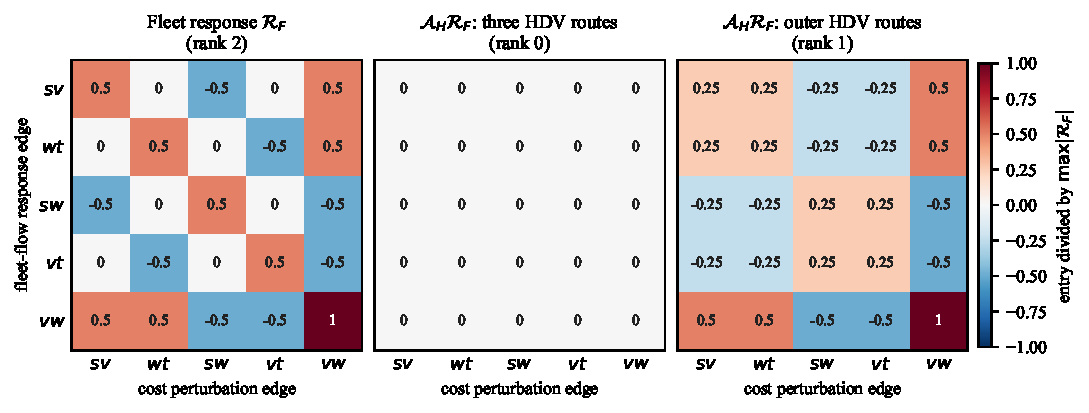
\includegraphics[width=\textwidth]{response_paper/figures/fig_braess_response_matrices.pdf}
\caption{Raw coalition response and HDV screening on the affine Braess network. Entries are normalized by the largest raw response entry. The coalition-side operator is held fixed across panels; changing only the HDV support changes the rank of the activated response.}
\label{fig:braess-response-matrices}
\end{figure}

\subsection{Sioux Falls: benchmarks and the conditional design criterion}

Sioux Falls has $76$ directed links and $528$ positive-demand OD pairs. The BPR benchmarks are $J^{UE}=7{,}480{,}226$ and $J^{SO}=7{,}194{,}256$, leaving a recoverable gap of $285{,}970$. Let $\mathfrak P(N)$ denote the set of partitions in the declared design menu and let $x^\ast(\Pi;\alpha,\gamma,\theta)$ be the certified continuation equilibrium under partition $\Pi$, AV penetration $\alpha$, coordination intensity $\gamma$, and objective-type vector $\theta$. The conditional design problem evaluated below is
\begin{equation}\label{eq:conditional-coalition-design}
 \Pi^\star(\alpha,\gamma,\theta)
 \in \arg\min_{\Pi\in\mathfrak P(N)}J\!\left(x^\ast(\Pi;\alpha,\gamma,\theta)\right).
\end{equation}
Equation~\eqref{eq:conditional-coalition-design} is an ex post design comparison over specified arrangements. It does not assign firms a payoff, permit deviations, or claim that the selected partition is stable.

\subsection{Objective composition at fixed concentration}\label{sec:sf-composition}

The first Sioux Falls experiment holds constant the quantities that a concentration statistic can see. Four equal-mass companies have objective types
\[
 (\tau_1,\tau_2,\tau_3,\tau_4)=(0.5,0.5,1.5,1.5),
\]
proportional but separately conserved OD obligations, company HHI $0.25$, two equal-mass coalitions, coalition HHI $0.5$, and identical route access. We compare assortative pairs $\{\{1,2\},\{3,4\}\}$ with mixed pairs $\{\{1,3\},\{2,4\}\}$. Only the composition of objective types within the coalitions changes.

\begin{table}[!htbp]
\centering
\small
\caption{Certified assortative-minus-mixed composition contrasts. Positive recovery differences favor assortative grouping; positive $\Delta J/J^{UE}$ means higher assortative TSTT.}
\label{tab:composition-contrast}
\begin{tabular}{ccrrrr}
\toprule
&&\multicolumn{2}{c}{$\alpha=0.5$}&\multicolumn{2}{c}{$\alpha=0.9$}\\
\cmidrule(lr){3-4}\cmidrule(lr){5-6}
$\gamma$&&$\Delta$ recovery (pp)&$\Delta J/J^{UE}$&$\Delta$ recovery (pp)&$\Delta J/J^{UE}$\\
\midrule
$0$    && $0.000$  & $0.0000\%$  & $0.000$  & $0.0000\%$\\
$0.25$ && $-0.294$ & $0.0112\%$  & $-1.285$ & $0.0491\%$\\
$0.50$ && $-1.168$ & $0.0446\%$  & $-1.161$ & $0.0444\%$\\
$0.75$ && $-0.244$ & $0.0093\%$  & $-0.228$ & $0.0087\%$\\
$1.00$ && $1.876$  & $-0.0717\%$ & $1.031$  & $-0.0394\%$\\
\bottomrule
\end{tabular}
\end{table}

At $\gamma=0$, the two partitions are invariant up to solver tolerance, as predicted by Proposition~\ref{prop:governance}. Once cross-member terms are active, the ordering changes with governance: mixed pairs close more of the recoverable gap at $\gamma=0.25$--$0.75$, whereas assortative pairs are better at $\gamma=1$. The largest baseline TSTT contrast is $0.0717\%$ of $J^{UE}$, so the effect is modest in absolute network time but decisive for the ordering of otherwise matched arrangements. This is a controlled identification result: an average objective type, coalition size, or HHI cannot recover the relevant response.

\begin{figure}[!htbp]
\centering
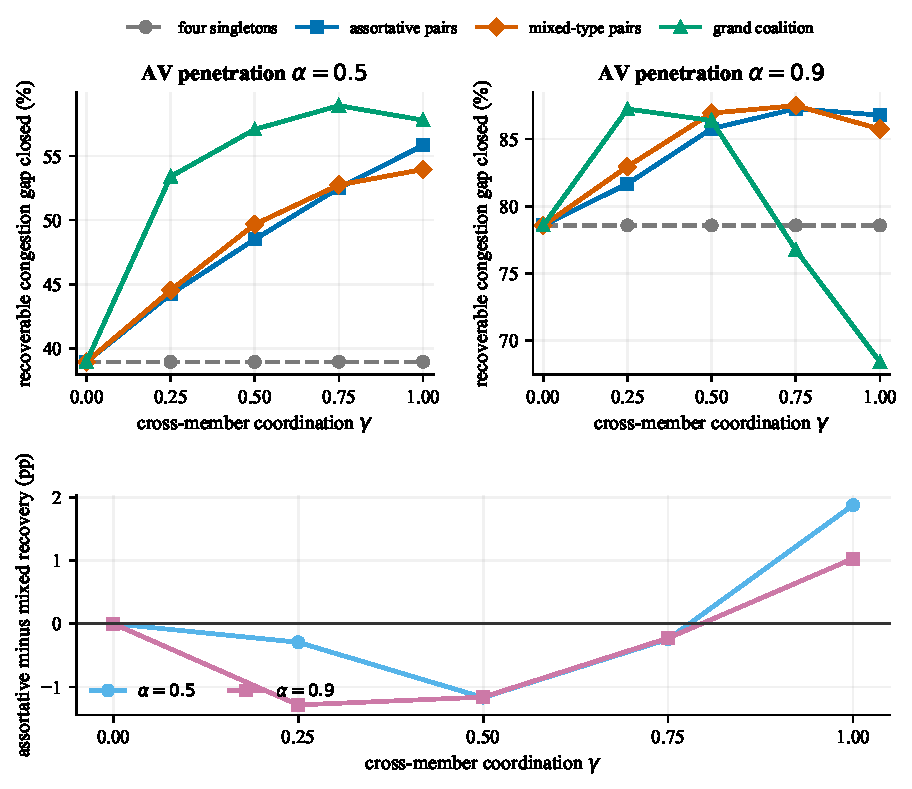
\includegraphics[width=\textwidth]{response_paper/figures/fig_sf_coalition_composition.pdf}
\caption{Coalition objective composition at fixed company masses, coalition sizes, OD obligations, and HHI. The top panels report recovery by partition; the bottom panel reports the assortative-minus-mixed recovery contrast.}
\label{fig:sf-composition}
\end{figure}

\subsection{State-contingent regimes in Sioux Falls}\label{sec:sf-design-map}

We evaluate all $15$ set partitions of the same four companies so that the
performance of any proposed selection rule can be measured against a known
benchmark. With $\varepsilon=10^{-8}$ in
\eqref{eq:epsilon-optimal-partitions}, Table~\ref{tab:best-partition} reports
the set of certified optima rather than forcing a numerical tie to be unique.

\begin{table}[!htbp]
\centering
\small
\caption{Set-valued optimum in the Sioux Falls $n=4$ audit scan. Company labels are one based. All comparisons use the same objective types, OD portfolios, route access, and identity-preserving governance rule.}
\label{tab:best-partition}
\begin{tabular}{ccp{5.0cm}rrr}
\toprule
$\alpha$ & $\gamma$ & $\varepsilon$-optimal partition set & $K$ & coalition HHI & gain vs. singleton (pp)\\
\midrule
0.5 & 0.5 & $\{\{1,2,3,4\}\}$ & 1 & 1.000 & 18.096\\
0.5 & 1.0 & $\{\{1,2,3,4\}\}$ & 1 & 1.000 & 18.810\\
0.9 & 0.5 & $\{\{1,2,3\}|\{4\},\ \{1,2,4\}|\{3\}\}$ & 2 & 0.625 & 8.745\\
0.9 & 1.0 & $\{\{1,2\}|\{3\}|\{4\}\}$ & 3 & 0.375 & 8.540\\
\bottomrule
\end{tabular}
\end{table}

The benchmark exhibits a clear state transition. At moderate AV penetration,
the grand coalition is optimal for both tested governance intensities. At high
penetration, partial coordination is optimal. The two three--one arrangements
at $\alpha=0.9,\gamma=0.5$ differ in TSTT by only $5.58\times10^{-7}$, or
$7.46\times10^{-12}J^{UE}$, because the two high-type companies are symmetric.
At $\gamma=1$, the optimum retains three decision centers. Thus stronger
governance does not imply that all companies should share one dispatcher. This
pattern is consistent with Theorem~\ref{thm:canonical-regimes}: coordination
should move the network toward its effective response target, which may lie at
an endpoint or in the interior.

\begin{figure}[!htbp]
\centering
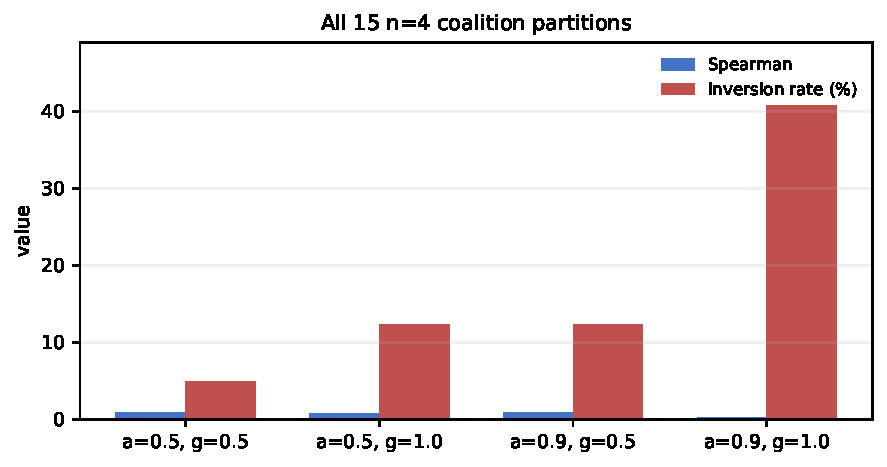
\includegraphics[width=0.9\textwidth]{response_paper/figures/fig_coalition_partition_scan.pdf}
\caption{Complete $n=4$ Sioux Falls audit scan. The exhaustive values establish the benchmark optimum used to evaluate local selection rules; they are not required by the rules themselves.}
\label{fig:coalition-partition-scan}
\end{figure}

\subsection{Local selection rules and policy regret}\label{sec:policy-regret}

For larger company sets, enumerating the Bell-number partition space is not a
practical design rule. We therefore test two agglomerative policies. The
one-step policy starts from singleton companies, evaluates every feasible
pairwise merge of the current blocks, chooses the best improving merge, and
stops when none improves TSTT. The two-step policy chooses the first merge on
the best improving path of length at most two. Both policies use only local
coarsenings of the current partition. The complete $n=4$ scans are retained
solely to calculate their ex post recovery regret
\begin{equation}\label{eq:policy-regret}
 \operatorname{Reg}(\widehat\Pi;s)
 :=100\frac{J(\widehat\Pi;s)-J^*(s)}{J^{UE}-J^{SO}}
 \quad\text{recovery percentage points}.
\end{equation}

\begin{table}[!htbp]
\centering
\small
\caption{Policy regret against the complete $n=4$ audit scans. Exact counts use the same relative TSTT tolerance as \eqref{eq:epsilon-optimal-partitions}.}
\label{tab:policy-regret}
\begin{tabular}{llrrr}
\toprule
benchmark & policy & exact states & mean regret (pp) & max regret (pp)\\
\midrule
Sioux Falls (4 states) & one-step merge & 4/4 & 0.000 & 0.000\\
 & two-step merge & 4/4 & 0.000 & 0.000\\
 & always grand & 2/4 & 4.908 & 18.695\\
 & always singleton & 0/4 & 13.548 & 18.810\\
\addlinespace
Braess and grid (32 states) & one-step merge & 29/32 & 0.332 & 8.339\\
 & two-step merge & 32/32 & 0.000 & 0.000\\
 & always grand & 27/32 & 1.520 & 18.205\\
 & always singleton & 0/32 & 21.752 & 42.289\\
\bottomrule
\end{tabular}
\end{table}

The one-step rule is exact in all Sioux Falls states and in $29$ of $32$
cross-network states, with mean regret $0.332$ points, but it has an $8.339$-point
failure on Braess at $\alpha=0.7,\gamma=0.75$. The other failures are $2.141$
points at $(0.9,0.5)$ and $0.130$ points at $(0.9,1)$. Two-step lookahead
repairs these local traps and reaches an $\varepsilon$-optimal arrangement in
all $36$ tested states. This is benchmark evidence, not a theorem of universal
optimality. For four companies the two-step neighborhood covers much of the
small partition lattice; for general $n$ it remains a local rule and avoids
requiring an ex ante enumeration of all Bell-number partitions.

\subsection{Governance-cost regimes}\label{sec:governance-cost-regimes}

The TSTT-minimizing organization need not be preferred once coordination
requires institutional resources. We apply \eqref{eq:penalized-coalition-loss}
to the Sioux Falls audit scan. At $\alpha=0.5,\gamma=1$, the lower envelope
passes through all four organizational degrees as $\lambda$ increases.

\begin{table}[!htbp]
\centering
\small
\caption{Governance-cost regimes at $\alpha=0.5,\gamma=1$. Endpoints are pairwise indifference thresholds; the displayed partition is optimal in the open interval.}
\label{tab:governance-regimes}
\begin{tabular}{lll r}
\toprule
$\lambda$ interval & selected partition & description & $K$\\
\midrule
$[0,0.0293)$ & $\{1,2,3,4\}$ & grand coalition & 1\\
$[0.0293,0.2678)$ & $\{1,2\}|\{3,4\}$ & two pairs & 2\\
$[0.2678,0.7435)$ & $\{1,2\}|\{3\}|\{4\}$ & one pair & 3\\
$[0.7435,\infty)$ & $\{1\}|\{2\}|\{3\}|\{4\}$ & singletons & 4\\
\bottomrule
\end{tabular}
\end{table}

The sequence is not imposed by a preference for intermediate structures. Each
partition supplies an equilibrium-congestion intercept and a governance-cost
slope; Proposition~\ref{prop:governance-cost-threshold} determines their
crossings. When coordination is inexpensive, the congestion gain justifies a
grand coalition. As the burden rises, partial coalitions retain the most
valuable internalization while avoiding some cross-company links. Fragmented
control becomes optimal only after the congestion benefit no longer covers the
governance burden.

\subsection{Cross-network validation of the regime transition}\label{sec:cross-network}

We repeat the complete $15$-partition audit on two independent BPR topologies:
a five-edge Braess network and a directed $3\times3$ grid with three ODs. The
design crosses four penetrations
$\alpha\in\{0.3,0.5,0.7,0.9\}$, four governance intensities
$\gamma\in\{0.25,0.5,0.75,1\}$, and the common objective vector
$(0.5,0.5,1.5,1.5)$. All $480=2\times4\times4\times15$ profiles pass the VI
and full-route oracle tests. The maximum VI gap is $9.971\times10^{-7}$ and
the maximum relative omitted-route slack is $3.79\times10^{-16}$.

\begin{table}[!htbp]
\centering
\small
\caption{Cross-network organizational regimes over 16 states per topology.}
\label{tab:cross-network-regimes}
\begin{tabular}{lrrl}
\toprule
network & grand-optimal states & partial-optimal states & transition at $\alpha=0.9$\\
\midrule
Braess & 14 & 2 & partial for $\gamma\in\{0.75,1\}$\\
directed grid & 13 & 3 & partial for $\gamma\in\{0.5,0.75,1\}$\\
\bottomrule
\end{tabular}
\end{table}

Both networks select the grand coalition in every tested state with
$\alpha\leq0.7$. At $\alpha=0.9$, sufficiently strong governance produces a
partial-coordination regime on both topologies, although the transition occurs
at a lower $\gamma$ on the grid. The qualitative state transition therefore
survives a change in topology, OD count, and cost calibration, while its
boundary remains network dependent.

\begin{figure}[!htbp]
\centering
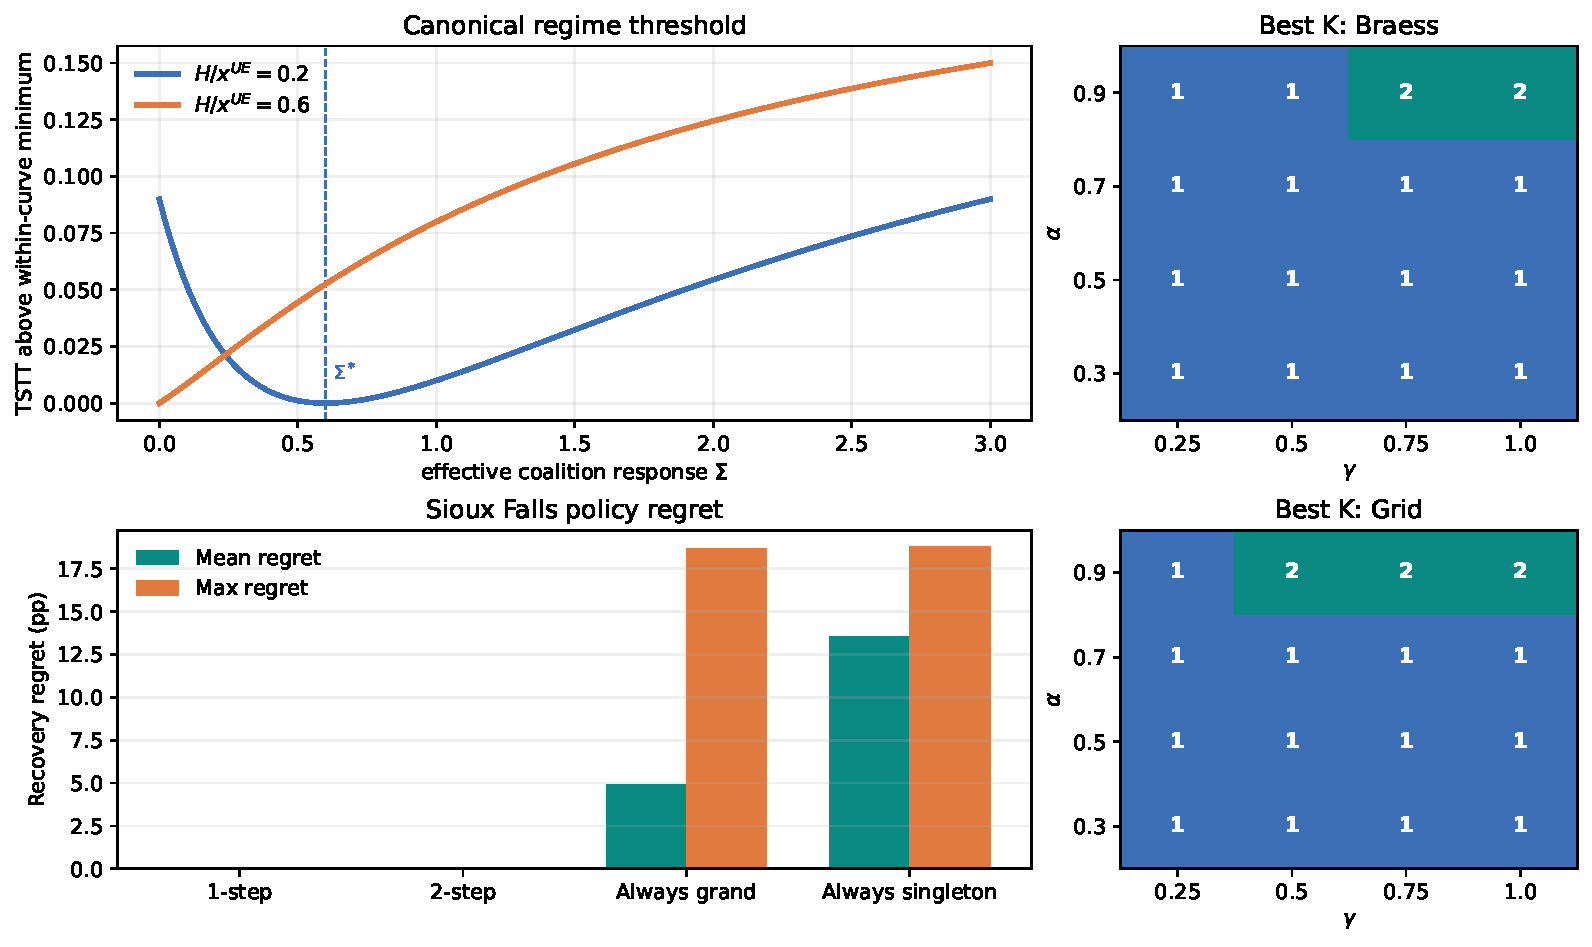
\includegraphics[width=\textwidth]{response_paper/figures/fig_regime_validation.pdf}
\caption{Regime theory and validation. The canonical bottleneck has an interior target $\Sigma^*$ only when $H<x^{UE}/2$; the Braess and grid heatmaps report the best coalition count; the Sioux Falls bars report policy regret.}
\label{fig:regime-validation}
\end{figure}

\subsection{Company count and coalition degree}\label{sec:sf-degree}

The degree scan varies the number of underlying companies $n\in\{2,4,8\}$ while holding total AV mass and aggregate demand fixed. Companies have equal mass within each $n$ and alternate low and high objective types. For each $n$, singleton, balanced intermediate, and grand-coalition partitions are compared within the same objective-type distribution.

\begin{table}[!htbp]
\centering
\small
\caption{Grand-minus-singleton coalition-degree effects at full cross-member coordination. Company HHI is descriptive; $K$ and $n$ are distinct organizational dimensions.}
\label{tab:degree-contrast}
\begin{tabular}{ccrrr}
\toprule
$\alpha$ & $n$ & $\rho_{K=1}-\rho_{K=n}$ (pp) & $\Delta J/J^{UE}$ & company HHI\\
\midrule
$0.5$ & $2$ & $1.956$ & $-0.075\%$ & $0.500$\\
$0.5$ & $4$ & $18.811$ & $-0.719\%$ & $0.250$\\
$0.5$ & $8$ & $29.489$ & $-1.127\%$ & $0.125$\\
$0.9$ & $2$ & $-18.365$ & $0.702\%$ & $0.500$\\
$0.9$ & $4$ & $-10.155$ & $0.388\%$ & $0.250$\\
$0.9$ & $8$ & $11.927$ & $-0.456\%$ & $0.125$\\
\bottomrule
\end{tabular}
\end{table}

At $\alpha=0.5$, the grand coalition improves recovery relative to singleton governance, with the effect increasing from $1.956$ to $29.489$ points as $n$ rises from $2$ to $8$. At $\alpha=0.9$, the same intervention is harmful for $n=2$ and $n=4$ but beneficial for $n=8$, ranging from $-18.365$ to $11.927$ points. Intermediate coordination is also material: at $\alpha=0.9$, moving from singletons to balanced pairs changes recovery by $7.179$ points for $n=4$ and $25.227$ points for $n=8$. The comparison makes clear why an ownership statistic cannot substitute for reporting both the underlying company count and the active coalition count.

\begin{figure}[!htbp]
\centering
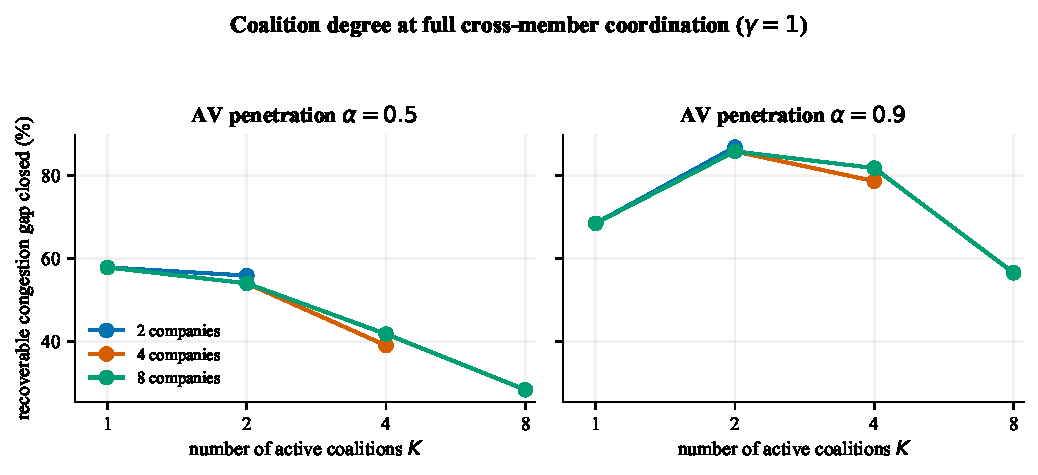
\includegraphics[width=0.95\textwidth]{response_paper/figures/fig_sf_coalition_degree.pdf}
\caption{Coalition degree at full cross-member coordination. Lines connect balanced partitions across the available coalition counts $K$ for each underlying company count $n$.}
\label{fig:sf-degree}
\end{figure}

\subsection{Sensitivity, audit diagnostics, and weak-effect boundaries}

The controlled composition comparison is repeated over objective-type gaps $\tau_H-\tau_L\in\{0.5,1.0,1.5\}$, reference management-slope scales $\{0.5,1,2\}\bar b$, five values of $\gamma$, and $\alpha\in\{0.5,0.9\}$. All $180$ profiles are certified. The two partitions coincide at $\gamma=0$ for every design. For $\gamma>0$, the contrast is generally nonzero but is not sign invariant. The absolute contrast reaches $9.089$ recovery points (wide gap, $\alpha=0.9$, unit slope scale). Sign reversals over $\gamma$ occur in multiple gap--scale combinations, including the baseline design. The robust statement is therefore behavioral: objective composition is active under coordination. No universal ranking of assortative and mixed grouping is supported.

\begin{table}[!htbp]
\centering
\small
\caption{Sensitivity summary for the assortative-minus-mixed recovery contrast. Each row aggregates five $\gamma$ values and is based on certified profiles.}
\label{tab:sensitivity-summary}
\begin{tabular}{cccrrr}
\toprule
$\alpha$ & type gap & slope scale & min contrast (pp) & max contrast (pp) & sign reversal\\
\midrule
0.5 & 0.5 & 0.5 & $-0.496$ & $0.210$ & yes\\
0.5 & 1.0 & 1.0 & $-1.168$ & $1.877$ & yes\\
0.5 & 1.5 & 1.0 & $-3.553$ & $0.000$ & no\\
0.9 & 0.5 & 1.0 & $-1.029$ & $0.018$ & yes\\
0.9 & 1.0 & 1.0 & $-1.285$ & $1.031$ & yes\\
0.9 & 1.5 & 1.0 & $-9.089$ & $0.000$ & no\\
\bottomrule
\end{tabular}
\end{table}

The complete $n=4$ scan also audits whether a mass statistic could substitute
for the response-based policy. All $15$ partitions are evaluated at
$\alpha\in\{0.5,0.9\}$ and $\gamma\in\{0.5,1\}$, yielding $60$ certified
profiles. At $\alpha=0.5$, coalition-HHI/recovery Spearman correlations are
$0.906$ and $0.793$ at $\gamma=0.5$ and $1$, with inversion rates $4.94\%$ and
$12.35\%$. At $\alpha=0.9$, the correlation falls from $0.815$ to $0.236$ and
the inversion rate rises from $12.35\%$ to $40.74\%$. The high-penetration,
full-coordination profiles span $0.684$--$0.871$ in recovery and $0.715\%$ of
$J^{UE}$ in TSTT. These are systematic within-benchmark diagnostics, not
population estimates. They explain why HHI is inadequate for selecting among
the candidate merges evaluated by the local policies.

\begin{table}[!htbp]
\centering
\small
\caption{All $n=4$ set-partition scan. Values are computed across the $15$ partitions in each condition.}
\label{tab:partition-scan}
\begin{tabular}{ccrrrr}
\toprule
$\alpha$ & $\gamma$ & Spearman & Kendall & inversion rate & recovery range\\
\midrule
0.5 & 0.5 & 0.906 & 0.807 & 4.94\% & $0.390$--$0.571$\\
0.5 & 1.0 & 0.793 & 0.671 & 12.35\% & $0.390$--$0.578$\\
0.9 & 0.5 & 0.815 & 0.671 & 12.35\% & $0.786$--$0.873$\\
0.9 & 1.0 & 0.236 & 0.165 & 40.74\% & $0.684$--$0.871$\\
\bottomrule
\end{tabular}
\end{table}

\begin{figure}[!htbp]
\centering
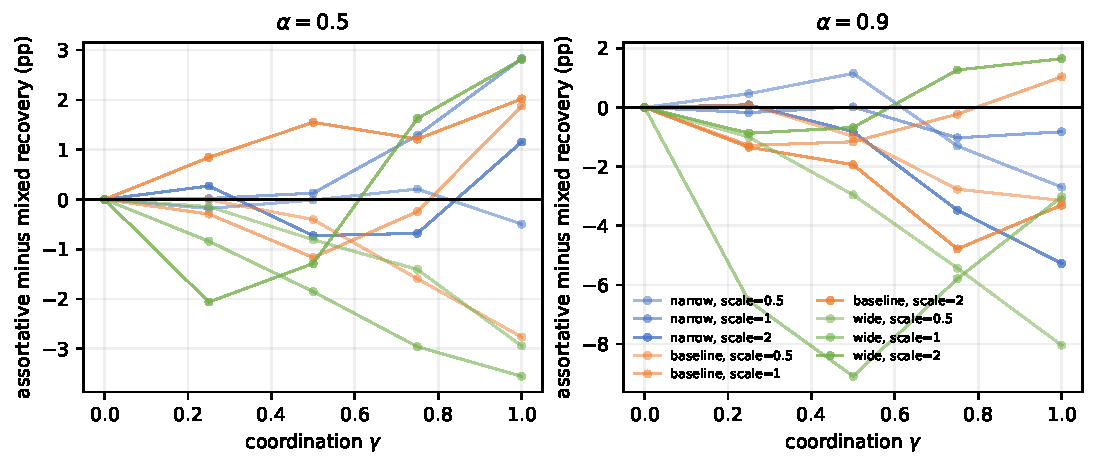
\includegraphics[width=\textwidth]{response_paper/figures/fig_coalition_sensitivity.pdf}
\caption{Objective-gap and governance-scale sensitivity. Lines report the certified assortative-minus-mixed recovery contrast over $\gamma$; colors denote objective gap and line opacity denotes reference-slope scale.}
\label{fig:coalition-sensitivity}
\end{figure}

\subsection{Spatial exposure and HDV penetration}

The fixed-HHI spatial experiment assigns four equal fleets the same total OD demand and company HHI $0.25$ but changes their spatial OD portfolios. Recovery spans $30.75\%$--$42.44\%$ at $\alpha=0.5$ and $10.15\%$--$74.33\%$ at $\alpha=0.9$. The largest displacement from proportional allocation is $0.363\%$ and $2.360\%$ of $J^{UE}$, respectively. Spatial exposure is therefore a design input alongside coalition size: identical masses can have different activated responses because they control different OD corridors.

\begin{figure}[!htbp]
\centering
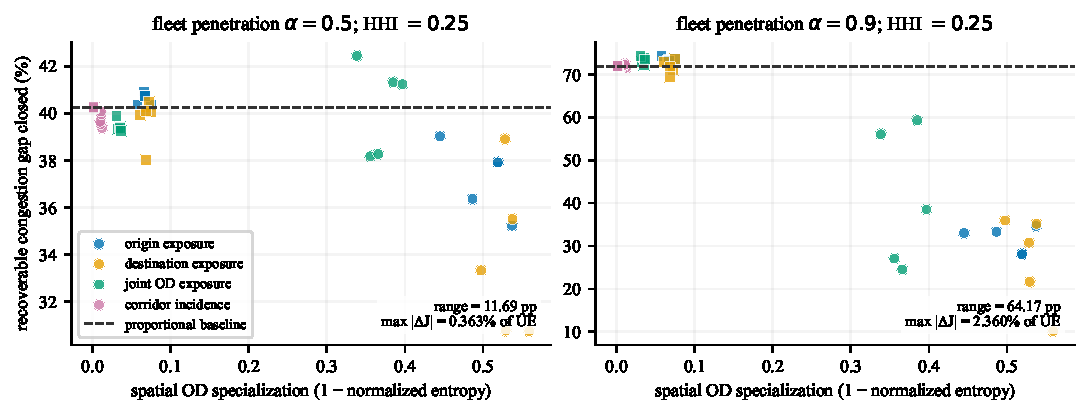
\includegraphics[width=\textwidth]{response_paper/figures/fig_sf_spatial_od.pdf}
\caption{Spatial OD portfolios change congestion at fixed equal fleet masses and HHI. The figure is a complementary exposure test, not a market-population estimate.}
\label{fig:sf-spatial}
\end{figure}

The penetration scan under common $\beta=1$ reports all-pair reversal rates of $18.10\%$, $18.73\%$, $10.65\%$, $10.14\%$, and $6.75\%$ at $\alpha=0.1,0.3,0.5,0.7,0.9$. Median reversal magnitudes range from $0.006\%$ to $0.043\%$ of $J^{UE}$. More HDVs can absorb a larger share of coalition displacement, reducing practical effect sizes; this transmission mechanism does not impose an ownership or coalition ordering. The earlier $200$-profile decomposition scan remains a robustness check: HHI--recovery Spearman correlations are $0.967$, $0.975$, and $0.988$ under the mass-linked prior, full-information $\beta=1$, and common $\beta=0.5$ regimes, with all-pair reversal rates $7.97\%$, $7.05\%$, and $4.14\%$. These proportional-portfolio results are secondary to the regime and policy analysis.

\subsection{Identity-preserving coordination versus operational pooling}

Pooling is a separate feasible-authority intervention, not another label for objective coordination. We compare the same two-coalition objective, company masses, aggregate OD demand, and $\gamma=1$ under identity-preserving and operational-pooling constraints. With proportional member OD portfolios and common route access, pooling changes member labels but not the induced aggregate route-flow set, as established in Proposition~\ref{prop:pooling}. Four certified profiles confirm the boundary: the largest pooling-minus-identity TSTT difference is $0.003$ time units, or $3.94\times10^{-10}J^{UE}$, and the largest recovery difference is $1.0308357\times10^{-6}$ percentage points. Pooling is neutral in this symmetric design. The result is a scope boundary, not evidence that pooling is neutral with heterogeneous route access or spatially specialized member portfolios.

\subsection{Summary of the evidence}

The experiments support a regime and policy conclusion rather than a universal
concentration law. Objective composition changes the coalition response only
when cross-member terms are active; OD portfolios and route geometry determine
where that response points; and HDV support determines how much reaches
aggregate congestion. The analytic bottleneck threshold explains why either
centralized or partial governance can be preferred. The cross-network scans
show the same broad transition from grand to partial coordination as AV
penetration and governance intensity rise, although the boundary is
topology-specific. A local one-step merge rule has low but nonzero regret, and
two-step lookahead reaches the audit optimum in all tested states. Governance
costs then generate explicit grand, partial, and fragmented intervals. The
result is a falsifiable selection framework for specified arrangements, not a
claim that firms will voluntarily form the selected coalition.

\section{Discussion: From Coalition Effects to Coalition Policy}\label{sec:discussion}

\subsection{The organizational question resolved by the model}

The paper begins with a routing-control question rather than a concentration
question. AV companies face a common physical congestion technology but can
use different management objectives for their controlled vehicles. Coalition
governance determines which of those objectives are optimized jointly and
which cross-member effects are internalized. Because each member retains its
accepted OD demand, an organizational change first alters an OD-feasible route
response. The road network maps that response into edge flows, and HDVs then
absorb the component they can reproduce through Wardrop reallocation. Only the
remaining activated response can change aggregate congestion.

This mechanism explains why coalition degree lacks a universal ordering. A
larger coalition need not generate a larger or more socially aligned activated
response. Its cross-member terms can rotate the response toward a different
set of congested edges, and HDV substitution can remove some directions but
not others. The relevant policy object is therefore the system-cost projection
of the screened response. Proposition~\ref{prop:merge-regimes} makes this
statement operational: a proposed increase in coupling improves TSTT when its
merge-direction score is negative, is neutral when the score is zero, and is
harmful when the score is positive.

\subsection{When centralization and partial independence are preferred}

The canonical theorem turns the general directional criterion into a regime
map. When interior HDVs can offset the coalition response, they pin the
congested route at the Wardrop flow and organization is locally neutral. Once
that screening support disappears, the fixed component $H$ and effective
coalition response $\Sigma$ determine system performance. If
$H\geq x^{UE}/2$, TSTT is nondecreasing in $\Sigma$, so a centralizing move is
desirable when it reduces effective response. If $H<x^{UE}/2$, system cost is
minimized at the interior target
$\Sigma^*=1-2H/x^{UE}$. A partial coalition can then dominate both complete
centralization and complete fragmentation because it produces a response
closer to the target.

The theorem does not assert that a merger always reduces $\Sigma$. That
relationship depends on the declared objective family and governance matrix.
It instead states a sharper condition: once the response induced by an
organization is known or estimated, the preferred direction follows from its
position relative to the active regime. On a general network, the scalar
target becomes the merge-direction score, which must be recomputed after a
support change.

\subsection{What the network evidence adds}

The Sioux Falls audit scan is consistent with the regime logic. At
$\alpha=0.5$, the grand coalition minimizes TSTT for both tested positive
governance intensities. At $\alpha=0.9$, the optimal set retains independent
decision centers: symmetry-equivalent three--one partitions at $\gamma=0.5$
and a two--one--one partition at $\gamma=1$. The two-network validation shows
the same qualitative transition. All tested Braess and grid states with
$\alpha\leq0.7$ select the grand coalition, whereas high penetration and
sufficiently strong governance produce partial optima on both networks. The
transition occurs at different values of $\gamma$, so topology changes the
boundary without eliminating the regime.

These results improve upon a list of partition rankings in two ways. First,
the analytic theorem explains why an interior organization can be optimal.
Second, policy regret asks whether a decision rule can recover the organization
without treating the full partition lattice as the prescription. One-step
merging is exact in all four Sioux Falls states and $29$ of $32$ cross-network
states, with only $0.332$ points of mean cross-network regret. Its three Braess
failures are informative: local improvement can stop before a jointly valuable
sequence of merges becomes visible. Two-step lookahead crosses these local
traps and reaches an audit optimum in all $36$ states. This observed exactness
does not establish universal optimality, particularly because the four-company
two-step neighborhood covers much of the small partition lattice.

\subsection{Governance burden changes the recommendation}

Minimizing TSTT alone treats coordination as costless. The burden model in
\eqref{eq:governance-burden} separates the network benefit from the resources
needed to maintain cross-company governance. Each arrangement then defines an
affine loss in $\lambda$: its congestion performance is the intercept and its
coordination burden is the slope. The lower envelope yields exact switching
thresholds. In the Sioux Falls example at $\alpha=0.5,\gamma=1$, the selected
organization moves from grand coordination to two pairs, then to one pair, and
finally to singletons as the governance-cost weight rises.

This result gives partial coalitions a substantive interpretation. They are not
arbitrary intermediate points or evidence that moderation is always best.
They appear when the marginal congestion benefit of an additional cross-member
link no longer covers its governance burden. Alternative cost functions could
change the thresholds or remove an intermediate interval; the lower-envelope
method remains valid once that burden is specified.

\subsection{Why HHI cannot implement the policy}

The response-based policy needs variables that a passive ownership cross
section does not reveal. The controlled composition experiment holds company
and coalition HHI, masses, coalition sizes, OD obligations, and route access
fixed, yet changing which objective types are grouped alters recovery and can
reverse the ordering along the governance path. Across the full Sioux Falls
audit, the coalition-HHI/recovery Spearman correlation falls to $0.236$ and the
pairwise inversion rate reaches $40.74\%$ at high penetration and full
governance. At fixed company HHI, changing spatial OD portfolios creates even
larger variation because it changes the network directions controlled by each
company.

HHI remains useful for describing the distribution of fleet mass. It cannot
select a coalition organization because it omits objective curvature,
cross-member governance, OD authority, route access, active support, and HDV
screening. The policy should therefore treat HHI as a screening covariate and
estimate or simulate the activated response directly.

\subsection{Observability and implementation}

Implementation requires four classes of inputs: accepted company-level OD
obligations, available routes or dispatch authority, calibrated physical delay
functions, and a defensible approximation of each company's marginal
management objective. Under a stable support, OD-preserving perturbations can
identify screened aggregate-flow responses and provide the ingredients for the
merge score. When supports change, the manager can use the certified
continuation solver to evaluate the local one- or two-step merge neighborhood.
This creates an auditable workflow: diagnose the response regime, evaluate
candidate local merges, report regret against richer audit scans when feasible,
and include governance burden before recommending an organization.

The recommendation applies to an operator, platform, or regulator that can
compare specified governance arrangements. It does not imply that every member
would accept the system-optimal continuation design. Private implementation
requires a payoff-allocation or transfer rule, contracting costs, deviation
protocols, and a partition-formation concept.

\subsection{Scope and limitations}

The exact response and regime results require affine physical costs, fixed
active supports, nonredundant OD tangents, and positive curvature on
coalition-feasible directions. The BPR experiments provide certified numerical
continuation equilibria, not a global nonlinear extension of the affine
theorem. The governance burden is a transparent sensitivity primitive rather
than an externally calibrated institutional cost. Objective types are also
controlled primitives; estimating them from operator dispatch data remains an
important empirical task.

The routing stage conditions on an externally realized batch of accepted
requests. Pricing, passenger choice, endogenous demand, empty-vehicle
repositioning, service quality, capacity and headway effects, private profit,
and endogenous coalition stability remain outside the model. The complete
partition scans cover four-company benchmark menus rather than a population of
markets, and the two-step policy has no general optimality guarantee. These
boundaries leave a clear next step: combine empirically identified objectives
with scalable local search and a partition-function formation game, while
retaining the continuation-equilibrium mechanism established here.

\section{Conclusion}\label{sec:conclusion}

This paper asks when heterogeneous AV companies should coordinate their
routing and when partial independence should be retained. Companies experience
the same physical road costs but can manage their fleets under different
objectives. A coalition aggregates those objectives and internalizes selected
cross-member effects while preserving member OD obligations; HDVs continue to
choose routes through a nonatomic Wardrop equilibrium. The resulting
organizational problem concerns the continuation congestion induced by a
specified coalition, not the ownership shares alone and not the private
stability of coalition formation.

The theory connects objective heterogeneity to a usable coalition-design
criterion. On a fixed affine support, the activated signature retains the
OD-feasible coalition response that survives HDV reallocation. Its projection
onto marginal system cost yields a general-network merge-direction score. The
canonical bottleneck exposes three regimes: HDV screening can make organization
neutral; a boundary regime favors changes that lower effective response; and
an interior-response regime can make partial coordination better than both
grand and singleton organization. Adding governance burden gives closed-form
pairwise thresholds and a lower envelope of grand, partial, and fragmented
policy intervals.

The certified experiments test both the regime and the selection rule. Sioux
Falls moves from a grand-coalition optimum at moderate penetration to partial
coordination at high penetration. Independent Braess and directed-grid scans
show the same qualitative transition, with topology-specific boundaries. A
one-step merge policy reaches an audit optimum in $33$ of $36$ total states and
has mean regret $0.332$ points on the $32$ cross-network states; two-step
lookahead reaches an audit optimum in all $36$. The latter result is evidence
within the declared four-company designs rather than a universal guarantee.
Objective-composition, company-count, spatial-exposure, and sensitivity tests
explain why the policy cannot be replaced by HHI or coalition count.

The practical conclusion is conditional but specific. A decision maker should
estimate or simulate the activated response, use its system-cost projection to
screen candidate merges, search a local merge neighborhood, and account for
the cost of cross-company governance. Centralization is justified when that
process moves the network toward its response target and the congestion gain
covers the coordination burden. Partial independence is justified when further
coupling overshoots the target or costs more than it saves. Extending this
continuation design to empirically calibrated objectives and endogenous
coalition formation is a separate research step.

\section*{Data Availability Statement}
All analytical derivations, experiment scripts, machine-readable result files, figure generators, and numerical validators used for this manuscript are included in the repository accompanying the paper. The Sioux Falls network inputs are identified in Appendix~\ref{app:sf-params}.

\section*{Ethics Statement}
This study uses public benchmark network data and controlled computational scenarios. It does not involve human participants, personal data, or animal subjects.

\section*{Author Contributions}
Luyao Niu: conceptualization, methodology, mathematical analysis, software, experiments, and writing. Ruolin Li: conceptualization, methodology, mathematical analysis, review, and writing.

\section*{Conflict of Interest}
The authors declare no conflict of interest.

\section*{Funding}
No external funding was received for this study.

\section*{AI-Assisted Writing Disclosure}
Generative AI tools were used for drafting assistance, code-review support, and language editing. The authors verified the mathematical derivations, experimental outputs, citations, and final manuscript and remain responsible for all content.
\appendix

\section{Additional Analytical Details}\label{app:analysis}

\subsection{Quadratic coalition objectives and private travel time}

This subsection clarifies the economic normalization behind the quadratic specification. The integral in \eqref{eq:coalition-objective} supplies the common marginal road cost. A quadratic term is then needed if the coalition is meant to internalize the delay generated by its own flow rather than merely take that delay as given.

For affine costs, the physical part of coalition $C$'s objective on edge $e$ is
\[
 \int_0^{F_e^C}[a_e+b_e(x_e^{-C}+s)]\,ds
 =a_eF_e^C+b_ex_e^{-C}F_e^C+\frac12b_e(F_e^C)^2.
\]
Coalition travel time on that edge is
\[
 F_e^C[a_e+b_e(x_e^{-C}+F_e^C)]
 =a_eF_e^C+b_ex_e^{-C}F_e^C+b_e(F_e^C)^2.
\]
Thus the management penalty $\frac12b_e(F_e^C)^2$ converts the physical integral into the coalition's private total travel time on that edge. The equality is a normalization for the affine case, not a claim that every application must use total travel time as its private objective. For a singleton, $F_e^C=f_e^i$. For a fully integrated identity-preserving coalition, the governance matrix $b_e\mathbf 1_C\mathbf 1_C^\top$ produces exactly this aggregate square. A diagonal matrix retains separate member objectives; off-diagonal elements add cross-member internalization. The general quadratic form in \eqref{eq:quadratic-objective} allows these terms to coexist with route-specific priorities $q_C$.

\subsection{Projected inverse in a null-space basis}

Let $Z_C$ have orthonormal columns spanning $\ker\Gamma_C$. Any feasible active flow is $y_C^0+Z_Cu$. The coalition's fixed-support quadratic first-order condition restricted to this tangent is
\[
 (Z_C^\top H_CZ_C)u
 =-Z_C^\top[H_Cy_C^0+\Lambda_C^\top(a+Bx)+q_C].
\]
The tangent positive-definiteness condition \eqref{eq:coalition-tangent-pd} makes the coefficient invertible and gives
\[
 P_C=Z_C(Z_C^\top H_CZ_C)^{-1}Z_C^\top.
\]
This formula remains valid when $H_C$ is singular on route-space directions that cannot be generated by an OD-preserving movement. Exact duplicate routes must be combined or quotiented out when they create a zero-curvature vector in $\ker\Gamma_C$. The condition is therefore a statement about curvature on feasible deviations, not a requirement that the primitive objective be strictly convex in every route coordinate.

\subsection{HDV projection identities}

The HDV block enters the theorem through feasible reallocation directions, not through an additional management objective. The matrix $\mathcal A_H$ removes the edge-flow component that HDVs can generate while preserving their OD totals and equal-cost condition.

Let $K_H=L_H^\top BL_H$. Under \eqref{eq:hdv-tangent-pd},
\[
 \mathcal A_H=I-L_HK_H^{-1}L_H^\top B.
\]
The identities in Lemma~\ref{lem:screening} follow from
\[
 \mathcal A_HL_H=L_H-L_HK_H^{-1}K_H=0
\]
and
\[
 \mathcal A_H^2
 =I-2L_HK_H^{-1}L_H^\top B
 +L_HK_H^{-1}K_HK_H^{-1}L_H^\top B
 =\mathcal A_H.
\]
If $\mathcal A_Hv=0$, then $v=L_HK_H^{-1}L_H^\top Bv$, proving $\ker\mathcal A_H=\range(L_H)$. Symmetry of $B$ and $K_H$ gives $\mathcal A_H^\top B=B\mathcal A_H$.

\subsection{BPR continuation diagnostic}

The fixed-reference BPR implementation used in the main experiments is a convex potential-based behavioral continuation model; it is not the exact nonlinear own-travel-time atomic game unless the physical slope is constant.

The exact activated-response theorem is affine. It should not be read as a closed-form solution for the BPR continuation game. For BPR costs, the monotonicity proof in Proposition~\ref{prop:coalition-monotone} applies directly because BPR costs are continuous and nondecreasing and the coalition management matrices are PSD. The earlier perceived-slope specification has a more restrictive pointwise symmetric-Jacobian condition. On one edge, with fleet flows $f^k$, coefficients $\beta_k$, and $x=\sum_kf^k+h$, the condition is
\begin{equation}\label{eq:bpr-exact-psd}
 \frac{c''(x)}{c'(x)}
 \sqrt{\sum_k\beta_k(f^k)^2}\leq2.
\end{equation}
For a BPR exponent $\eta>1$, a readily checked sufficient bound is
\begin{equation}\label{eq:bpr-coarse-psd}
 \beta_{\max}\sigma\leq\frac{4}{(\eta-1)^2},
 \qquad \sigma=\max_k f^k/x.
\end{equation}
At $\eta=4$ the threshold is $4/9$. A pointwise pass records membership in a sufficient region; a fail removes that guarantee but is not evidence of multiplicity. All BPR profiles in the paper are certified independently by VI residual and omitted-route tests. Those numerical certificates establish approximate equilibrium of the solved route-generation problem; they do not extend the affine signature theorem to nonlinear BPR costs.

\subsection{Symbolic check of the canonical regime derivative}

For the bottleneck theorem, substituting
$x_1=(H+\Sigma x^{UE})/(1+\Sigma)$ into
$J=Na+t_1(x_1^2-x^{UE}x_1)$ and differentiating gives
\[
 \frac{dJ}{d\Sigma}
 =t_1(2x_1-x^{UE})\frac{x^{UE}-H}{(1+\Sigma)^2}.
\]
The identity
\[
 2x_1-x^{UE}=\frac{2H+(\Sigma-1)x^{UE}}{1+\Sigma}
\]
then yields \eqref{eq:bottleneck-tstt-derivative}. The repository script
\texttt{verify\_regime\_theorem.py} checks this simplification symbolically
and records the zero residual and threshold in
\texttt{regime\_theorem\_verification.json}. The script is a reproducibility
check; the proof in Theorem~\ref{thm:canonical-regimes} supplies the
mathematical argument.

\section{Sioux Falls Data and Numerical Certification}\label{app:sf-params}

Sioux Falls has $24$ nodes, $76$ directed links, and $528$ positive-demand OD pairs. Demand, free-flow times, and capacities are read from the standard network files in the repository. Total demand is $360{,}600$. Physical costs use \eqref{eq:bpr}. The all-HDV user-equilibrium and system-optimum TSTTs are $7{,}480{,}226$ and $7{,}194{,}256$, respectively.

The initial route set contains the three shortest free-flow routes per OD. It is expanded by player-specific shortest-path column generation, because a route that is unattractive at free flow can become attractive under the marginal objective induced by coalition governance. A route is added when its current marginal route cost is below the minimum held-route marginal cost by more than $10^{-6}$ times the route-cost scale. The VI is solved with adaptive Korpelevich extragradient and Euclidean projection onto each identity-preserving company--OD simplex. The accepted profiles satisfy normalized VI gap at most $10^{-6}$ and full-network omitted-route slack at most $10^{-6}$.

The composition experiment contains $40$ profiles for four equal-mass
companies with objective types $(0.5,0.5,1.5,1.5)$. It crosses two penetration
values, five coordination values, and four partitions. The degree experiment
contains $54$ profiles across $n\in\{2,4,8\}$, two penetration values, three
coordination values, and all declared balanced partitions.

The sensitivity experiment contains $180$ profiles crossing three objective gaps, three reference-slope scales, five coordination values, two penetrations, and the assortative/mixed partition pair. The complete $n=4$ partition scan contains all $15$ set partitions at two positive coordination values and two penetrations, for $60$ profiles. The pooling decomposition contains four profiles comparing identity-preserving and operational-pooling feasibility. All $338$ Sioux Falls coalition-extension profiles are certified.

The cross-network audit contains a five-edge Braess topology and a directed
$3\times3$ grid with three positive-demand ODs. For each topology, the design
crosses four AV penetration levels, four governance intensities, and all $15$
partitions of four companies, for $480$ profiles. All profiles are certified;
the maximum normalized VI gap is $9.971\times10^{-7}$ and the maximum relative
omitted-route slack is $3.79\times10^{-16}$. The raw profile file is
\texttt{cross\_network\_regime\_results.json}; the state and policy summaries
are in \texttt{cross\_network\_regime\_summary.json}.

Policy regret is computed after, rather than during, equilibrium solution.
\nolinkurl{coalition_design_analysis.py} calculates set-valued Sioux Falls
optima, one- and two-step merge paths, fixed-policy regret, and the
governance-cost lower envelope. \nolinkurl{cross_network_policy_analysis.py}
applies the same local policies to the two independent topologies. The
validator \nolinkurl{validate_regime_package.py} checks profile counts,
certification thresholds, finiteness, Sioux Falls policy consistency, and the
reported cross-network regret values.

The fixed-HHI spatial experiment contains $82$ certified profiles. Four equal-mass companies have HHI $0.25$ at both $\alpha=0.5$ and $0.9$; iterative proportional fitting preserves every aggregate OD row and every fleet-mass column while varying spatial OD portfolios. The response-decomposition experiment contains $600$ certified rows, the penetration scan $500$, and the targeted BPR audit $10$. The raw and summary JSON files, scripts, and validators are included in the repository.

\begin{table}[htbp]
\centering
\scriptsize
\setlength{\tabcolsep}{3pt}
\caption{Numerical certification summary. All rows satisfy both acceptance criteria. Exact PSD entries are pointwise diagnostics for the earlier perceived-slope family, not acceptance criteria for the new coalition quadratic family.}
\label{tab:certificates}
\begin{tabular}{lcccr}
\toprule
Experiment & certified & max VI gap & max relative oracle slack & rows\\
\midrule
coalition composition & $40/40$ & $1.0\times10^{-6}$ & $1.0\times10^{-6}$ & 40\\
coalition degree & $54/54$ & $9.97\times10^{-7}$ & $9.91\times10^{-7}$ & 54\\
coalition sensitivity & $180/180$ & $1.0\times10^{-6}$ & $1.0\times10^{-6}$ & 180\\
all $n=4$ partitions & $60/60$ & $1.0\times10^{-6}$ & $1.0\times10^{-6}$ & 60\\
Braess/grid regime audit & $480/480$ & $9.97\times10^{-7}$ & $3.79\times10^{-16}$ & 480\\
identity/pooling decomposition & $4/4$ & $9.84\times10^{-7}$ & $3.2\times10^{-8}$ & 4\\
fixed-HHI spatial OD & $82/82$ & $1.0\times10^{-6}$ & $1.0\times10^{-6}$ & 82\\
response decomposition & $600/600$ & $1.0\times10^{-6}$ & $9.0\times10^{-7}$ & 600\\
penetration scan & $500/500$ & $1.0\times10^{-6}$ & $4.2\times10^{-7}$ & 500\\
BPR anchor audit & $10/10$ & $1.0\times10^{-6}$ & $1.2\times10^{-7}$ & 10\\
\bottomrule
\end{tabular}
\end{table}

\section{Reproducibility and Scope Ledger}\label{app:reproducibility}

The current coalition solver extends the previous fleet solver through optional coalition governance arguments while preserving the earlier model as a default nested case. The coalition objective uses fixed reference curvature $\bar b_e=c'_e(x_e^{UE})$ and the PSD matrix in \eqref{eq:gamma-governance}. The company-count scan uses equal company masses within each $n$ and holds total AV mass fixed across $n$. Singleton profiles at nonzero $\gamma$ are generated from the analytically verified partition invariance at $\gamma=0$; they are labeled as derived rows in the raw JSON and are not counted as independent solver runs. These implementation choices define the declared counterfactual menu; they do not estimate how firms would choose a coalition in an unfixed market.

The empirical claims in Section~\ref{sec:experiments} are limited to the declared Sioux Falls benchmark and governance design. The objective types are controlled primitives, not estimates from operator data. Operational pooling, endogenous coalition stability, transfers, pricing, passenger choice, and platform welfare remain outside the reported core results. The theoretical claims are likewise conditional: existence and monotonicity use continuous nondecreasing physical costs, whereas the activated signature and its minimality use affine costs, fixed supports, and the stated tangent-rank conditions.

The repository includes the extension and cross-network scripts, raw and
summary JSON outputs, symbolic checks, fail-closed validators, and
figure-generation code. Pooling is implemented as a coalition-level simplex
over member-route coordinates; its comparison with identity-preserving
coordination is interpreted only under the proportional OD and common-route
design reported in Section~\ref{sec:experiments}. The local merge policies use
full scans only as audit baselines for regret. Their zero observed two-step
regret is not encoded as an assumption and is not claimed as a general
optimality theorem.


\bibliographystyle{plainnat}
\bibliography{refs}

\end{document}
